\documentclass[12pt]{article}
\usepackage{xr-hyper}
\usepackage[unicode]{hyperref}

% \usepackage[hyphens]{url}
\usepackage[dvipsnames,svgnames,x11names]{xcolor}
\usepackage{amsmath,amssymb}
\usepackage{iftex}
\ifPDFTeX
  \usepackage[T1]{fontenc}
  \usepackage[utf8]{inputenc}
  \usepackage{textcomp} % provide euro and other symbols
\else % if luatex or xetex
  \usepackage{unicode-math}
  \defaultfontfeatures{Scale=MatchLowercase}
  \defaultfontfeatures[\rmfamily]{Ligatures=TeX,Scale=1}
\fi
\usepackage{lmodern}
\ifPDFTeX\else  
    % xetex/luatex font selection
\fi
% Use upquote if available, for straight quotes in verbatim environments
\IfFileExists{upquote.sty}{\usepackage{upquote}}{}
\IfFileExists{microtype.sty}{% use microtype if available
  \usepackage[]{microtype}
  \UseMicrotypeSet[protrusion]{basicmath} % disable protrusion for tt fonts
}{}
\makeatletter
\@ifundefined{KOMAClassName}{% if non-KOMA class
  \IfFileExists{parskip.sty}{%
    \usepackage{parskip}
  }{% else
    \setlength{\parindent}{0pt}
    \setlength{\parskip}{6pt plus 2pt minus 1pt}}
}{% if KOMA class
  \KOMAoptions{parskip=half}}
\makeatother
\usepackage{xcolor}
\setlength{\emergencystretch}{3em} % prevent overfull lines
\setcounter{secnumdepth}{5}
% Make \paragraph and \subparagraph free-standing
\makeatletter
\ifx\paragraph\undefined\else
  \let\oldparagraph\paragraph
  \renewcommand{\paragraph}{
    \@ifstar
      \xxxParagraphStar
      \xxxParagraphNoStar
  }
  \newcommand{\xxxParagraphStar}[1]{\oldparagraph*{#1}\mbox{}}
  \newcommand{\xxxParagraphNoStar}[1]{\oldparagraph{#1}\mbox{}}
\fi
\ifx\subparagraph\undefined\else
  \let\oldsubparagraph\subparagraph
  \renewcommand{\subparagraph}{
    \@ifstar
      \xxxSubParagraphStar
      \xxxSubParagraphNoStar
  }
  \newcommand{\xxxSubParagraphStar}[1]{\oldsubparagraph*{#1}\mbox{}}
  \newcommand{\xxxSubParagraphNoStar}[1]{\oldsubparagraph{#1}\mbox{}}
\fi
\makeatother


\providecommand{\tightlist}{%
  \setlength{\itemsep}{0pt}\setlength{\parskip}{0pt}}\usepackage{longtable,booktabs,array}
\usepackage{calc} % for calculating minipage widths
% Correct order of tables after \paragraph or \subparagraph
\usepackage{etoolbox}
\makeatletter
\patchcmd\longtable{\par}{\if@noskipsec\mbox{}\fi\par}{}{}
\makeatother
% Allow footnotes in longtable head/foot
\IfFileExists{footnotehyper.sty}{\usepackage{footnotehyper}}{\usepackage{footnote}}
\makesavenoteenv{longtable}
\usepackage{graphicx}
\makeatletter
\def\maxwidth{\ifdim\Gin@nat@width>\linewidth\linewidth\else\Gin@nat@width\fi}
\def\maxheight{\ifdim\Gin@nat@height>\textheight\textheight\else\Gin@nat@height\fi}
\makeatother
% Scale images if necessary, so that they will not overflow the page
% margins by default, and it is still possible to overwrite the defaults
% using explicit options in \includegraphics[width, height, ...]{}
\setkeys{Gin}{width=\maxwidth,height=\maxheight,keepaspectratio}
% Set default figure placement to htbp
\makeatletter
\def\fps@figure{htbp}
\makeatother

\addtolength{\oddsidemargin}{-.5in}%
\addtolength{\evensidemargin}{-.1in}%
\addtolength{\textwidth}{1in}%
\addtolength{\textheight}{1.7in}%
\addtolength{\topmargin}{-1in}
\makeatletter
\@ifpackageloaded{caption}{}{\usepackage{caption}}
\AtBeginDocument{%
\ifdefined\contentsname
  \renewcommand*\contentsname{Table of contents}
\else
  \newcommand\contentsname{Table of contents}
\fi
\ifdefined\listfigurename
  \renewcommand*\listfigurename{List of Figures}
\else
  \newcommand\listfigurename{List of Figures}
\fi
\ifdefined\listtablename
  \renewcommand*\listtablename{List of Tables}
\else
  \newcommand\listtablename{List of Tables}
\fi
\ifdefined\figurename
  \renewcommand*\figurename{Figure}
\else
  \newcommand\figurename{Figure}
\fi
\ifdefined\tablename
  \renewcommand*\tablename{Table}
\else
  \newcommand\tablename{Table}
\fi
}
\@ifpackageloaded{float}{}{\usepackage{float}}
\floatstyle{ruled}
\@ifundefined{c@chapter}{\newfloat{codelisting}{h}{lop}}{\newfloat{codelisting}{h}{lop}[chapter]}
\floatname{codelisting}{Listing}
\newcommand*\listoflistings{\listof{codelisting}{List of Listings}}
\makeatother
\makeatletter
\makeatother
\makeatletter
\@ifpackageloaded{caption}{}{\usepackage{caption}}
\@ifpackageloaded{subcaption}{}{\usepackage{subcaption}}
\makeatother


\ifLuaTeX
  \usepackage{selnolig}  % disable illegal ligatures
\fi
\usepackage[]{natbib}
\bibliographystyle{apalike}
\usepackage{bookmark}

\IfFileExists{xurl.sty}{\usepackage{xurl}}{} % add URL line breaks if available
\urlstyle{same} % disable monospaced font for URLs
\hypersetup{
  pdftitle={Title},
  pdfauthor={Author 1; Author 2},
  pdfkeywords={3 to 6 keywords, that do not appear in the title},
  colorlinks=true,
  linkcolor={blue},
  filecolor={Maroon},
  citecolor={Blue},
  urlcolor={Blue},
  pdfcreator={LaTeX via pandoc}}

\newcommand{\anon}{0}

%set the key \texttt{anon} to ``0'' to hide the authors and acknowledgements,
%  producing the required anonymized version. 
%Set the key \texttt{anon} to ``1'' to produce the manuscript with author details and
% acknowledgments. 

% Add additional packages here if required
\usepackage{siunitx}

% document
% \usepackage{geometry}
% \setlength{\parindent}{0pt}
% \setlength{\parskip}{1em}
% \renewcommand{\baselinestretch}{1}
% \usepackage[raggedright]{titlesec}

% grafics
\usepackage{graphicx}
\graphicspath{ {./images/sa/} }
\usepackage[export]{adjustbox}
\usepackage{caption}
\usepackage{subcaption}

\usepackage{rotating}
\renewcommand{\topfraction}{.85}
\renewcommand{\bottomfraction}{.7}
\renewcommand{\textfraction}{.15}
\renewcommand{\floatpagefraction}{.66}
\renewcommand{\dbltopfraction}{.66}
\renewcommand{\dblfloatpagefraction}{.66}
\setcounter{topnumber}{9}
\setcounter{bottomnumber}{9}
\setcounter{totalnumber}{20}
\setcounter{dbltopnumber}{9}

\usepackage{tikz}
\usepackage{tkz-graph}  
\usetikzlibrary{shapes.geometric}
\usetikzlibrary{bayesnet, positioning}
\tikzset{ % Define edge styles
    solid edge/.style={->, thick, color=black},
    dashed edge/.style={->, dashed, color=black},
}

% math and text
\usepackage{bm}
\usepackage{mathtools}
\usepackage{amsthm}
\usepackage{nicematrix}

\usepackage[section]{placeins}
\newcommand*{\vertbar}{\rule[-1ex]{0.5pt}{2.5ex}}
\newcommand*{\horzbar}{\rule[.5ex]{2.5ex}{0.5pt}}
\usepackage{xcolor}
\usepackage{tcolorbox}
\usepackage[inline]{enumitem}
\usepackage{soul}

% tables
\usepackage{booktabs}
\usepackage{multirow}
\usepackage{tabularx} 

% circulant notation
\newcommand{\mycirc}[1] {\underline{\bm{#1}}}
\newcommand{\mybcirc}[1] {\underline{\underline{\bm{#1}}}}

% matrix exponential symbol
\newcommand{\eP}{\hspace*{0.015cm}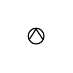
\begin{tikzpicture}[scale=0.1]
      \draw (0,0) circle(1.0);
      \draw (-0.85,-0.4) -- (0,0.9) -- (0.85,-0.4);
    \end{tikzpicture}\hspace*{0.015cm}}

% % algorithms
% \usepackage{algorithm}
% \usepackage{algorithmic}
% \usepackage{float}
% \newfloat{algorithm}{t}{lop}
% algorithms 
\usepackage[ruled,vlined]{algorithm2e}
\SetAlgoNlRelativeSize{0}    % smaller line numbers if needed
\SetAlgoCaptionSeparator{.}  % cleaner caption formatting
\SetAlgoNlRelativeSize{-1}   % even smaller line numbers (optional)


% % External refs
% \externaldocument{main}
% External refs
\makeatletter
\let\XR@bibcite\bibcite
\let\XR@citation\citation
\let\XR@bibdata\bibdata
\let\XR@bibstyle\bibstyle

\renewcommand{\bibcite}[2]{}
\renewcommand{\citation}[1]{}
\renewcommand{\bibdata}[1]{}
\renewcommand{\bibstyle}[1]{}

\externaldocument{main}

\let\bibcite\XR@bibcite
\let\citation\XR@citation
\let\bibdata\XR@bibdata
\let\bibstyle\XR@bibstyle
\makeatother

\begin{document}


\def\spacingset#1{\renewcommand{\baselinestretch}%
{#1}\small\normalsize} \spacingset{1}

%%%%%%%%%%%%%%%%%%%%%%%%%%%%%%%%%%%%%%%%%%%%%%%%%%%%%%%%%%%%%%%%%%%%%%%%%%%%%%


\if0\anon
{
  \title{Bayesian Semi-Blind Deconvolution at Scale}
  \author{
    Guillermina Senn$^{1}$,
    Håkon Tjelmeland$^{1}$,
    Nathan Glatt-Holtz$^{2}$, \\
    Matt Walker$^{3}$,
    and Andrew Holbrook$^{4}$\\[0.5em]
    $^{1}$Department of Mathematical Sciences, NTNU\\
    $^{2}$Indiana University\\
    $^{3}$BP\\
    $^{4}$Department of Biostatistics, UCLA
    }
    \date{}
  \maketitle
  % \thispagestyle{empty}
} \fi

\if1\anon
{
  \bigskip
  \bigskip
  \bigskip
  \begin{center}
    {\LARGE\bf Bayesian Semi-Blind Deconvolution at Scale}
    \end{center}
  \medskip
} \fi

\setcounter{figure}{0}
\setcounter{equation}{0}
\setcounter{section}{0}
\pagenumbering{arabic}
\setcounter{page}{1}
\renewcommand{\thesection}{S.\arabic{section}}
\renewcommand{\theequation}{S.\arabic{equation}}


\begin{center}
    {\large \bf SUPPLEMENTARY MATERIAL}
\end{center} 

% \newpage 
\spacingset{1.75} % DON'T change the spacing!

\section{Equivalence of certain Gaussian densities} \label{sec:equal_densities}
In this section, we show that $q(\bm{x}_u^{\star})=p(\bm{x}^{\star})$ as stated in Section~\ref{sec:preliminaries} in the main text. 
Following the setup in Section~\ref{sec:preliminaries}, let $\bm{x}^{\star} \sim N_n(\tilde{\bm{\mu}}, \tilde{\bm{\Sigma}})$ with density $p(\cdot)$ and let $\bm{x}_u^{\star} = \bm{A}^C \bm{x}^{\star} \sim N_{n-k}(\bm{A}^C \tilde{\bm{\mu}}, \bm{A}^C \tilde{\bm{\Sigma}} \bm{A}^{C^{\top}})$ with density $q(\cdot)$. 

Let
\begin{equation} \label{eq:density_p}
    p(\bm{x}^{\star}) := (2\pi)^{-(n-k)/2} |\tilde{\bm{\Sigma}}|^{-1/2}
    \exp{ \{-\frac{1}{2} (\bm{x}^{\star} - \tilde{\bm{\mu}})^{\top} (\tilde{\bm{\Sigma}})^{-} (\bm{x}^{\star} - \tilde{\bm{\mu}}) \}},
\end{equation}
where $|\tilde{\bm{\Sigma}}|$ denotes the pseudodeterminant and $\tilde{\bm{\Sigma}}^{-}$ the pseudoinverse of the singular, rank-$(n-k)$ matrix $\tilde{\bm{\Sigma}}$. 
Let 
\begin{equation} \label{eq:density_q}
\begin{split}
    q(\bm{x}_u^{\star}) &:= (2\pi)^{-(n-k)/2} |\bm{A}^C \tilde{\bm{\Sigma}} \bm{A}^{C^{\top}}|^{-1/2} \\
    &\times \exp{\{-\frac{1}{2} (\bm{A}^C \bm{x}^{\star} - \bm{A}^C \tilde{\bm{\mu}})^{\top} (\bm{A}^C \tilde{\bm{\Sigma}} \bm{A}^{C^{\top}})^{-1} (\bm{A}^C\bm{x}^{\star} - \bm{A}^C \tilde{\bm{\mu}})\}}.
\end{split}
\end{equation}

Now assume without loss of generality that the elements in $\bm{x}^{\star}$ are arranged such that the first $n-k$ elements correspond to the unconstrained elements, and the last $k$ elements to the constrained elements. Then  $\bm{A}^{C} = \begin{bmatrix}
    \bm{I}_{n-k} & \bm{0}_{n-k,k}
\end{bmatrix}$.
The order of the elements in $\bm{x}^{\star}$ lets us write the singular matrix $\tilde{\bm{\Sigma}}$ as the block matrix
\begin{equation} \label{eq:Sigma_star}
    \tilde{\bm{\Sigma}} = 
    \begin{bmatrix}
        \bm{\Sigma}_{1} & \bm{0}_{n-k, k} \\
        \bm{0}_{k, n-k} & \bm{0}_{k, k} 
    \end{bmatrix}.
\end{equation}
with $\bm{\Sigma}_{1}$ the full-rank $(n-k) \times (n-k)$ covariance matrix for the unconstrained elements. This gives $\bm{A}^C \tilde{\bm{\Sigma}} \bm{A}^{C^{\top}}=\bm{\Sigma}_{1}$ in~\eqref{eq:density_p}. The matrix $\bm{\Sigma}_{1}$ has therefore inverse $\bm{\Sigma}_{1}^{-1}$ and determinant $|\bm{\Sigma}_{1}| = \prod_{i=0}^{n-k-1}{\lambda_i}$, with $\lambda_i$ the $n-k$ eigenvalues of $\bm{\Sigma}_{1}$.

We now prove $q(\bm{x}_u^{\star})=p(\bm{x}^{\star})$ by showing that each factor in~\eqref{eq:density_p} is equal to each factor in~\eqref{eq:density_q}. The pseudodeterminant $|\tilde{\bm{\Sigma}}|$ in~\eqref{eq:density_p} is defined to be the product of the non-zero eigenvalues of $\tilde{\bm{\Sigma}}$. Thus, it is clear from~\eqref{eq:Sigma_star} that $|\tilde{\bm{\Sigma}}|=\prod_{i=0}^{n-k-1}{\lambda_i}=|\bm{\Sigma}_{1}|$. To show that the products inside the exponential terms in~\eqref{eq:density_p} and~\eqref{eq:density_q} are equal, rewrite the product in~\eqref{eq:density_q} as
\begin{equation*}
\begin{split}
    (\bm{A}^C \bm{x}^{\star} - \bm{A}^C \tilde{\bm{\mu}})^{\top} (\bm{A}^C \tilde{\bm{\Sigma}} \bm{A}^{C^{\top}})^{-1}& \\
    \times (\bm{A}^C\bm{x}^{\star} - \bm{A}^C \tilde{\bm{\mu}}) &= 
    (\bm{x}^{\star} - \tilde{\bm{\mu}})^{\top} \bm{A}^{C^{\top}}(\bm{A}^C \tilde{\bm{\Sigma}} \bm{A}^{C^{\top}})^{-1} \bm{A}^C (\bm{x}^{\star} - \tilde{\bm{\mu}}).
\end{split}
\end{equation*}


% old
% We now prove $q(\bm{x}_u^{\star})=p(\bm{x}^{\star})$ by showing that each factor in~\eqref{eq:density_p} is equal to each factor in~\eqref{eq:density_q}. The pseudodeterminant $|\tilde{\bm{\Sigma}}|$ in~\eqref{eq:density_q} is defined to be the product of the non-zero eigenvalues of $|\tilde{\bm{\Sigma}}|$. Thus, it is clear from~\eqref{eq:Sigma_star} that $|\tilde{\bm{\Sigma}}|=\prod_{i=0}^{n-k-1}{\lambda_i}=|\bm{\Sigma}_{1}|$. 

% To show that the product multiplications inside the expnential terms in~\eqref{eq:density_p} and~\eqref{eq:density_q} are equal, rewrite the product in~\eqref{eq:density_q} as
% \begin{equation*}
% \begin{split}
%     (\bm{A}^C \bm{x}^{\star} - \bm{A}^C \bm{\mu})^{\top} (\bm{A}^C \tilde{\bm{\Sigma}} \bm{A}^{C^{\top}})^{-1}& \\
%     \times (\bm{A}^C\bm{x}^{\star} - \bm{A}^C \bm{\mu}) &= 
%     (\bm{x}^{\star} - \bm{\mu})^{\top} \bm{A}^{C^{\top}}(\bm{A}^C \tilde{\bm{\Sigma}} \bm{A}^{C^{\top}})^{-1} \bm{A}^C (\bm{x}^{\star} - \bm{\mu}).
% \end{split}
% \end{equation*}

Then, showing that
\begin{equation}
\begin{split}
    (\bm{x}^{\star} - \tilde{\bm{\mu}})^{\top} \bm{A}^{C^{\top}}(\bm{A}^C \tilde{\bm{\Sigma}} \bm{A}^{C^{\top}})^{-1} \bm{A}^C (\bm{x}^{\star} - \tilde{\bm{\mu}})
    &= 
    (\bm{x}^{\star} - \tilde{\bm{\mu}})^{\top} (\tilde{\bm{\Sigma}})^{-} (\bm{x}^{\star} - \tilde{\bm{\mu}}),
\end{split}
\end{equation}
is equivalent to showing that
\begin{equation} \label{eq:intermediate_matrix_equality}
\begin{split}
    (\tilde{\bm{\Sigma}})^{-} = \bm{A}^{C^{\top}}(\bm{A}^C \tilde{\bm{\Sigma}} \bm{A}^{C^{\top}})^{-1} \bm{A}^C.
\end{split}
\end{equation}
Since $\bm{A}^{C} \bm{A}^{C^{\top}} = \bm{I}_{n-k}$, from~\eqref{eq:intermediate_matrix_equality} we have
\begin{equation} \label{eq:intermediate_matrix_equality2}
\begin{split}
    \bm{A}^C(\tilde{\bm{\Sigma}})^{-}\bm{A}^{C^{\top}} = (\bm{A}^C \tilde{\bm{\Sigma}} \bm{A}^{C^{\top}})^{-1}.
\end{split}
\end{equation}
From~\eqref{eq:Sigma_star}, the RHS of~\eqref{eq:intermediate_matrix_equality2} evaluates to $(\bm{A}^C \tilde{\bm{\Sigma}} \bm{A}^{C^{\top}})^{-1} = \bm{\Sigma}_1^{-1}$. Next, show that the LHS of~\eqref{eq:intermediate_matrix_equality2} also evaluates to $\bm{A}^C(\tilde{\bm{\Sigma}})^{-}\bm{A}^{C^{\top}} = \bm{\Sigma}_1^{-1}$. 

Let $\bm{G}$ denote the pseudoinverse $(\tilde{\bm{\Sigma}})^{-}$. This pseudoinverse is the block-matrix
\begin{equation}
    \bm{G} = 
    \begin{bmatrix}
        \bm{G}_{11} & \bm{G}_{12}\\
        \bm{G}_{21} & \bm{G}_{22} 
    \end{bmatrix},
\end{equation}
with conformable blocks. The pseudoinverse properties state that $\bm{G}$ is a pseudoinverse for $\tilde{\bm{\Sigma}}$ if and only if $\tilde{\bm{\Sigma}} = \tilde{\bm{\Sigma}} \bm{G} \tilde{\bm{\Sigma}}$. We then compute the block-product
\begin{equation}
\begin{split}
    \tilde{\bm{\Sigma}} \bm{G} \tilde{\bm{\Sigma}} 
    &= 
    \begin{bmatrix}
        \bm{\Sigma}_{1} & \bm{0}_{n-k, k} \\
        \bm{0}_{k, n-k} & \bm{0}_{k, k} 
    \end{bmatrix}
    \begin{bmatrix}
        \bm{G}_{11} & \bm{G}_{12}\\
        \bm{G}_{21} & \bm{G}_{22} 
    \end{bmatrix}
    \begin{bmatrix}
        \bm{\Sigma}_{1} & \bm{0}_{n-k, k} \\
        \bm{0}_{k, n-k} & \bm{0}_{k, k} 
    \end{bmatrix} \\
    &= 
    \begin{bmatrix}
        \bm{\Sigma}_1 \bm{G}_{11} \bm{\Sigma}_1 & \bm{0}_{n-k, k} \\
        \bm{0}_{k, n-k} & \bm{0}_{k, k} 
    \end{bmatrix}, 
\end{split}
\end{equation}
which implies that $\bm{\Sigma}_1 =  \bm{\Sigma}_1\bm{G}_{11} \bm{\Sigma}_1$ and in turn that $\bm{G}_{11}$ is a pseudoinverse for $\bm{\Sigma}_1$. Since $\bm{\Sigma}_1$ is invertible, and the pseudoinverse of an invertible matrix is the (unique) inverse of the matrix, $\bm{G}_{11} = \bm{\Sigma}_1^{-1}$. Finally, the LHS of~\eqref{eq:intermediate_matrix_equality2} evaluates to $\bm{A}^C(\tilde{\bm{\Sigma}})^{-}\bm{A}^{C^{\top}} = \bm{A}^C \bm{G} \bm{A}^{C^{\top}} = \bm{\Sigma}_1^{-1}$, giving the desired result. 
\qed

\section{A Kronecker product-based formula for \texorpdfstring{$\tilde{\bm{\Sigma}}_c$}{Sigma-tilde c}} \label{ap:refl_covariance}
The goal here is to write the covariance matrix $\tilde{\bm{\Sigma}}_c$ in~\eqref{eq:Sigma_c_star} of the constrained image prior in~\eqref{eq:image_constrained_prior} as a sum of Kronecker products.
Let $\bm{A}_{c, h}$ be a $1 \times n_h$ selection matrix for the columns of the extended lattice where pixels have been observed exactly. We next make the assumption that, for all these columns, the same rows have been observed, and define the $m \times n_v$ selection matrix $\bm{A}_{c, v}$ for these rows. Then the $m \times n$ constraint matrix $\bm{A}_c$ that selects the $m$ exact image observations from the extended image vector $\bm{c}$ is the Kronecker product $\bm{A}_c = \bm{A}_{c, h} \otimes \bm{A}_{c, v}$.

We next use that now both $\mybcirc{\Sigma}_c$ in~\eqref{eq:covariance_c} and $\bm{A}_c$ are Kronecker products to write the second term of $\tilde{\bm{\Sigma}}_c$ in~\eqref{eq:Sigma_c_star} as the Kronecker product $\sigma_c^2\bm{R}_{c, h}^{\star} \otimes  \bm{R}_{c, v}^{\star}$, with the Kronecker factors $\bm{R}_{c, h}^{\star}$ and $\bm{R}_{c, v}^{\star}$ given by 
\begin{equation} \label{eq:R_c_hv_star}
\begin{aligned}
    \bm{R}_{c, h}^{\star} &= (\mycirc{R}_{c, h}\bm{A}_{c, h}^{\top}) (\bm{A}_{c, h} \mycirc{R}_{c, h} \bm{A}_{c, h}^{\top})^{-1} (\bm{A}_{c, h} \mycirc{R}_{c, h}), \\
    \bm{R}_{c, v}^{\star} &=(\mycirc{R}_{c, v} \bm{A}_{c, v}^{\top})(\bm{A}_{c, v}\hspace*{0.07cm} \mycirc{R}_{c, v} \bm{A}_{c, v}^{\top})^{-1}(\bm{A}_{c, v} \mycirc{R}_{c, v}),
\end{aligned}
\end{equation}
which in turn gives
\begin{equation} \label{eq:Sigma_c_star_efficient_si}
\begin{split}
    \tilde{\bm{\Sigma}}_c
    &=  \sigma_c^2 \left( \mycirc{R}_{c, h} \otimes  \mycirc{R}_{c, v}  - \bm{R}_{c, h}^{\star} \otimes  \bm{R}_{c, v}^{\star} \right).
\end{split}
\end{equation}

% \subsection{Gradient of the log-determinant}
% To obtain $\dot{\bm{\Lambda}}^{i}_{\mybcirc{W}}$, recall that  $\mycirc{W}_0 = \mbox{circ}(\mycirc{P}\bm{w}^{\star})$, and then 
% \begin{equation}
%     \frac{\partial \mycirc{W}_0}{\partial w_i^{\star}} 
%     = \frac{\partial }{\partial w_i^{\star}} \mbox{circ}(\mycirc{P} \bm{w}^{\star})
%     = \mbox{circ}(\frac{\mycirc{P} \partial \bm{w}^{\star}}{\partial w_i^{\star}}) = 
%     \mbox{circ}(\mycirc{P}\bm{e}_i),
%     % = \bm{F}_{n_v}^H \dot{\bm{\Lambda}}^{i}_{\mycirc{W}_{0}} \bm{F}_{n_{v}}
% \end{equation}
% where $\bm{e}_i$ is the $i$-th standard vector.
% From the base-eigenvalue relation in~\eqref{eq:eigenvalues_fft_matrix}, 
% \begin{equation}
%     \mycirc{P}\bm{e}_i = \bm{F}_{n_{v}}^H \dot{\bm{\lambda}}_{\mycirc{W}_{0}}
%     \iff 
%     \dot{\bm{\lambda}}_{\mycirc{W}_{0}} = \bm{F}_{n_{v}} \mycirc{P}\bm{e}_i,
% \end{equation}
% where $\dot{\bm{\lambda}}_{\mycirc{W}_{0}}$ is the vector of eigenvalues, and then
% \begin{equation} \label{eq:derivative_W0}
%     \frac{\partial \mycirc{W}_0}{\partial w_i^{\star}} = \bm{F}_{n_{v}}^H \dot{\bm{\Lambda}}^{i}_{\mycirc{W}_{0}} \bm{F}_{n_{v}}
% \end{equation}
% where 
% $\dot{\bm{\Lambda}}^{i}_{\mycirc{W}_{0}}=\mbox{diag}(\dot{\bm{\lambda}}_{\mycirc{W}_{0}})$. 
% We now recall that $\mybcirc{W} = \bm{I}_{n_{h}} \otimes \mycirc{W}_0$.
% Then, using derivative rules and~\eqref{eq:derivative_W0},
% \begin{equation}
% \begin{split}
%     \frac{\partial \mybcirc{W}}{\partial w_i^{\star}}  
%     &= \bm{I}_{n_{h}} \otimes (\bm{F}_{n_{v}}^H \dot{\bm{\Lambda}}^{i}_{\mycirc{W}_{0}} \bm{F}_{n_{v}}) \\
%     &= (\bm{F}_{n_{h}} \otimes \bm{F}_{n_{v}})^H (\bm{I}_{n_{h}} \otimes \dot{\bm{\Lambda}}^{i}_{\mycirc{W}_{0}}) (\bm{F}_{n_{h}} \otimes \bm{F}_{n_{v}})\\
%     &= (\bm{F}_{n_{h}} \otimes \bm{F}_{n_{v}})^H \dot{\bm{\Lambda}}^{i}_{\mybcirc{W}} (\bm{F}_{n_{h}} \otimes \bm{F}_{n_{v}}).
% \end{split}
% \end{equation}

% We here explain how we applied the matrix derivatives and product rules in the Fourier domain to obtain $\dot{\bm{\Lambda}}_{\mybcirc{Z}}^{i}$.
% From~\eqref{eq:det_Y_derivative}, 
% \begin{equation} \label{eq:der_Z}
% \begin{split}
%     \frac{\partial \mybcirc{Z}}{\partial w_i^{\star}} 
%     &= \mybcirc{\Sigma}_c 
%     \left( \frac{\partial}{\partial w_i^{\star}} \; \mybcirc{W}^{\top} \mybcirc{A}^{-1}\mybcirc{W} \right) 
%     \mybcirc{\Sigma}_c
%     \iff
%     \dot{\bm{\Lambda}}_{\mybcirc{Z}}^{i} = \sigma_c^4 \bm{\Lambda}_{R_{c}}^2 \dot{\bm{\Lambda}}_{\mybcirc{W}^{\top}\mybcirc{A}^{-1}\mybcirc{W}}^{i}
%     % = -\bm{L}^{\top} \bm{A}_c^{\top} \frac{\partial \mybcirc{Z}}{\partial \omega_i} \bm{A}_c \bm{L}.
% \end{split}
% \end{equation}
% From the product rule,
% \begin{equation} \label{eq:derivative_WAW}
% \begin{split}
%     \frac{\partial}{\partial w_i^{\star}} \; \mybcirc{W}^{\top} \mybcirc{A}^{-1}\mybcirc{W}
%     &= \left(\frac{\partial \mybcirc{W}}{\partial w_i^{\star}}\right)^{\!T} 
%     \mybcirc{A}^{-1}\mybcirc{W}
%     + \mybcirc{W}^{\top} 
%     \left(\frac{\partial \mybcirc{A}^{-1}}{\partial w_i}\right)
%     \mybcirc{W}
%     + \mybcirc{W}^{\top} \mybcirc{A}^{-1} 
%     \left(\frac{\partial \mybcirc{W}}{\partial w_i}\right),
% \end{split}
% \end{equation}
% or in the Fourier domain
% \begin{equation}
%     \dot{\bm{\Lambda}}_{\mybcirc{W}^{\top}\mybcirc{A}^{-1}\mybcirc{W}}^{i} 
%     = \dot{\bm{\Lambda}}_{\mybcirc{W}}^{i^{H}} \bm{\Lambda}_{\mybcirc{A}}^{-1} \bm{\Lambda}_{\mybcirc{W}} + \bm{\Lambda}_{\mybcirc{W}}^H \dot{\bm{\Lambda}}_{\mybcirc{A}^{-1}}^{i} \bm{\Lambda}_{\mybcirc{W}} +
%     \bm{\Lambda}_{\mybcirc{W}}^H \bm{\Lambda}_{\mybcirc{A}}^{-1}
%     \dot{\bm{\Lambda}}_{\mybcirc{W}}^{i}
% \end{equation}
% where
% \begin{equation} \label{eq:derivative_inv_A}
% \begin{split}
%     \frac{\partial \mybcirc{A}^{-1}}{\partial w_i^{\star}} 
%     &= -\mybcirc{A}^{-1} 
%     \left(\frac{\partial \mybcirc{A}}{\partial w_i^{\star}}\right) 
%     \mybcirc{A}^{-1}
%     \iff
%     \dot{\bm{\Lambda}}_{\mybcirc{A}^{-1}}^{i} = -\bm{\Lambda}_{\mybcirc{A}}^{-2} \dot{\bm{\Lambda}}_{\mybcirc{A}}^{i},
% \end{split}
% \end{equation}
% with
% \begin{equation} \label{eq:derivative_A}
% \begin{split}
%     \frac{\partial \mybcirc{A}}{\partial w_i^{\star}} 
%     &= \left(\frac{\partial \mybcirc{W}}{\partial w_i^{\star}}\right) \mybcirc{\Sigma}_{c} \, \mybcirc{W}^{\top} 
%     + \mybcirc{W} \, \mybcirc{\Sigma}_{c} \left(\frac{\partial \mybcirc{W}}{\partial w_i^{\star}}\right)^{\!T} 
%     \iff
%     \dot{\bm{\Lambda}}_{\mybcirc{A}}^{i} = \sigma_c^2 \bm{\Lambda}_{R_{c}} \bigl( \dot{\bm{\Lambda}}^{i}_{\mybcirc{W}}  \bm{\Lambda}_{\mybcirc{W}}^H + 
%     \bm{\Lambda}_{\mybcirc{W}}
%     \dot{\bm{\Lambda}}_{\mybcirc{W}}^{i^{H}} \bigr)
% \end{split}
% \end{equation}

% \subsection{Gradient of the sum of squares}
% The expressions for $\mycirc{D}_i$ and $\bm{D}_i^{\star}$ are:
% \begin{equation*}
% \begin{aligned}
% \mycirc{D}_{ i} &= \mycirc{W}_0 \, \mycirc{R}_{c, v} \, (\partial \mycirc{W}_0 / \partial w_i^{\star})^{\top} + (\partial \mycirc{W}_0 / \partial w_i^{\star}) \, \mycirc{R}_{c, v} \, \mycirc{W}_0^{\top}, \\
% \bm{D}_{i}^{\star} &= \mycirc{W}_0 \, \bm{R}_{c, v}^{\star} \, (\partial \mycirc{W}_0 / \partial w_i^{\star})^{\top} +  (\partial \mycirc{W}_0 / \partial w_i^{\star}) \, \bm{R}_{c, v}^{\star T} \, \mycirc{W}_0^{\top}.   
% \end{aligned}
% \end{equation*}
% Computing $\bm{D}_i^{\star}$ has a cost of $\mathcal{O}(n_v^2 \log{n_v})$ and is done with traditional matrix multiplication.
% Computing $\mycirc{D}_i$ is done in the Fourier domain, 
% \begin{equation*}
%     \bm{\Lambda}_{\mycirc{D}_i} 
%     = (\dot{\bm{\Lambda}}_{\mycirc{W}_0}^{i}  \bm{\Lambda}_{\mycirc{R}_{c, v}} \bm{\Lambda}_{\mycirc{W}_0}^{H})^H
%     +  \dot{\bm{\Lambda}}_{\mycirc{W}_0}^{i}  \bm{\Lambda}_{\mycirc{R}_{c, v}} \bm{\Lambda}_{\mycirc{W}_0}^{H}.
% \end{equation*}

% Assuming that the transformed $\hat{\bar{\bm{d}}}$ is available, the vector $\bm{q}$ is computed as
% \begin{equation*}
%     \bm{q} = \bm{A}_c \mybcirc{B}^{\top} \bar{\bm{d}} = \bm{A}_c \mbox{IDFT2}(\bm{\Lambda}_{\mybcirc{B}} \hat{\bar{\bm{d}}}),
% \end{equation*}
% with complexity $\mathcal{O}(n \log n)$, where $\bm{\Lambda}_{\mybcirc{B}} = \sigma_c^2 \bm{\Lambda}_{R_{c}} \bm{\Lambda}_{\mybcirc{W}}^H \bm{\Lambda}_{\mybcirc{A}}^{-1}$ from the definition $\mybcirc{B} = \mybcirc{\Sigma}_c \mybcirc{W}^{\top} \mybcirc{A}^{-1}$.

% Assuming that the $m \times 1$ vector $\bm{S}^{-1}\bm{q}$ and the transformed $\hat{\bar{\bm{d}}}$ are available, the vector $\bm{v} = \bm{\Sigma}_{d|\omega}^{-1}\bar{\bm{d}}$ is computed in $\mathcal{O}(n\log n)$ as
% \begin{equation} \label{eq:v_computation}
% \begin{split}
%     \bm{v} 
%     &= \mybcirc{A}^{-1}\bar{\bm{d}}  + \mybcirc{B} \bm{A}_c^{\top} \bm{S}^{-1} \bm{A}_c \mybcirc{B}^{\top}\bar{\bm{d}} \\
%     &= \mbox{IDFT2}(\bm{\Lambda}_{\mybcirc{A}}^{-1} \hat{\bar{\bm{d}}}  + \bm{\Lambda}_{\mybcirc{B}} \odot \mbox{DFT2}(\bm{A}_c^{\top} \bm{S}^{-1} \bm{q})),
% \end{split}
% \end{equation}
% where in the first line we have replaced with the efficient expression~\eqref{eq:inv_sigmadw_1} for $\bm{\Sigma}_{d|\omega}^{-1}$ and the second line follows from circulant matrix algebra. Its transform $\hat{\bm{v}}$ is therefore the argument of the RHS of~\eqref{eq:v_computation}.


\section{Permutation matrix for the 1D circular convolution} \label{ap:permutation}
Let $\mycirc{P}=[P_{ij}]$ be the (circulant) permutation matrix that produces $\mycirc{P}\bm{x}$ to have the elements in a length-$n_v$ vector $\bm{x}$ first reversed in order and then circularly shifted $n_v/2$ positions upwards so that the first element of the vector $\mycirc{P}\bm{x}$ is the $n_v/2$-th element of $\bm{x}$. 
More precisely, the matrix $\mycirc{P}$ has all elements in the $\pm n_v/2$ diagonals equal to one, and all other elements equal to zero.
Then left-multiplying a length-$n_v$ vector with the circulant matrix $\mbox{circ}(\mycirc{P} \bm{x})$ 
performs the 1D circular convolution between $\bm{x}$ and the vector. 


\section{Full conditional distributions in the Gibbs sampler}\label{ap:gibbs}
In this section we describe how to efficiently sample from the full conditional distributions for $\bm{\omega}$, $\bm{c}_u^{\star}$, $\bm{d}_u^{\star}$, $\sigma_c^2$, and $\zeta$, obtained from the posterior in~\eqref{eq:posterior_cyclic} in the main text. 

\subsection{Full conditional for the image}\label{ap:fc_refl}
We sample from~\eqref{eq:FC_reflectivity_constrained} with CBK as follows. 
From the convolutional model in~\eqref{eq:blind_deconvolution}, $\bm{d}$ is a linear combination of the elements in $\bm{c}$, and therefore the joint distribution of $\bm{c}$ and $\bm{d}$ conditional on $\bm{\omega}, \sigma_w^2, \sigma_c^2, \zeta$ is given by
\begin{equation} \label{eq:joint_cd}
    \begin{pmatrix} \bm{c} \\ \bm{d}\end{pmatrix} | \bm{\omega}, \sigma_w^2, \sigma_c^2, \zeta 
    \sim N_{2n}(
    \begin{pmatrix} \bm{0} \\ \bm{0}\end{pmatrix}, \quad
    \begin{pmatrix} 
    \mybcirc{\Sigma}_c & \mybcirc{\Sigma}_c \, \mybcirc{W}^{\top}  \\ 
    \mybcirc{W} \, \mybcirc{\Sigma}_c  & \mybcirc{W} \,  \mybcirc{\Sigma}_c \, \mybcirc{W}^{\top}  + \mybcirc{\Sigma}_d
    \end{pmatrix} ),
\end{equation}
with conditional distribution given in~\eqref{eq:image_prior}
with parameters
\begin{align}\label{eq:image_fc_unc_params}
    \bm{\mu}_{c|d} &= \mybcirc{\Sigma}_c \hspace*{0.07cm}\mybcirc{W}^{\top} (\mybcirc{W} \hspace*{0.07cm} \mybcirc{\Sigma}_c \hspace*{0.07cm} \mybcirc{W}^{\top} + \mybcirc{\Sigma}_d)^{-1}\bm{d}, \\
    \mybcirc{\Sigma}_{c|d} &= \mybcirc{\Sigma}_c - \mybcirc{\Sigma}_c\hspace*{0.07cm} \mybcirc{W}^{\top} (\mybcirc{W}\hspace*{0.07cm} \mybcirc{\Sigma}_c\hspace*{0.07cm} \mybcirc{W}^{\top} + \mybcirc{\Sigma}_d)^{-1} \mybcirc{W}\hspace*{0.07cm} \mybcirc{\Sigma}_c
\end{align}
obtained with~\eqref{eq:gaussian_conditional_pars} from~\eqref{eq:joint_cd}. The density of the distribution in~\eqref{eq:fc_image_unconstrained} we denote by $p(\bm{c}| \bm{d}, \bm{\omega}, \sigma_c^2, \sigma_w^2, \zeta)$. 
Both $\mybcirc{\Sigma}_{c|d}$ and $\bm{\mu}_{c|d}$ can be obtained directly in the Fourier domain in $\mathcal{O}(n)$ with formulas~\eqref{eq:image_fc_unc_params_FD} in the main text, 
and a sample $\widehat{\bm{c}}$ from~\eqref{eq:fc_image_unconstrained} is obtained directly in the Fourier domain in $\mathcal{O}(n)$ with Algorithm~\ref{alg:fft_2d_mvn_FD}.

The CBK step that yields the corrected sample $\bm{c}^{\star} = \bm{c} | \{ \bm{A}_c \bm{c} = \bm{c}_o\}$ in the time domain is done with
\begin{equation} \label{eq:image_cbk_sample}
    \bm{c}^{\star} = \bm{c} -  \mybcirc{\Sigma}_{c|d} \,\bm{A}_c^{\top} (\bm{A}_c \, \mybcirc{\Sigma}_{c|d} \, \bm{A}_c^{\top})^{-1} (\bm{A}_c \bm{c} - \bm{c}_{o}),
\end{equation}
where the inverse transform $\bm{c} = \bm{F}_n^{-1}\widehat{\bm{c}}$ and the base of $\mybcirc{\Sigma}_{c|d}$ obtained from~\eqref{eq:image_fc_unc_params_FD} have a cost $\mathcal{O}(n \log n)$, the products  $\bm{A}_c \, \mybcirc{\Sigma}_{c|d}$ and $\bm{A}_c \, \mybcirc{\Sigma}_{c|d} \, \bm{A}_c^{\top}$ are built by simply picking out the right elements of the base of $\mybcirc{\Sigma}_{c|d}$, and assuming the number of constraints $m\ll n$, \eqref{eq:image_cbk_sample} can be done with traditional matrix operations with complexity $\mathcal{O}(m^3)$. 

\subsection{Blur full conditional} \label{ap:fc_blur}
As explained in Section~\ref{sec:fc_blur} in the main text, 
$\bm{w}|\bm{d} \sim N_{n_v}(\bm{\mu}_{w|d}, \mycirc{\Sigma}_{w|d})$
with conditional parameters $\bm{\mu}_{w|d}$ and $\mycirc{\Sigma}_{w|d}$
computed with~\eqref{eq:gaussian_conditional_pars}. 
Next, the Woodbury identity is used to rewrite the conditional covariance in~\eqref{eq:fc_blur_pars} as
\begin{align}\label{eq:fc_blur_cov_woodbury}
    \mycirc{\Sigma}_{w|d}= \bigl(\frac{\mycirc{R}_w^{-1}}{\sigma_w^2}+\frac{\bm{\Gamma}^{\top}\mybcirc{R}_d^{-1}\bm{\Gamma}}{\sigma_d^2} \bigr)^{-1}.
\end{align}

Noticing that $\bm{\Gamma}$ can be expressed as
\begin{equation}
    \bm{\Gamma} = (\bm{I}_{n_{h}} \otimes \bm{F}_{n_v}^H) \tilde{\bm{\Lambda}}_{\Gamma} \bm{F}_{n_v},
\end{equation}
where in a slight abuse of notation we use $\tilde{\bm{\Lambda}}_{\Gamma}$ to denote the $n_v \times n_h$ block matrix of diagonal eigenvalue matrices
\begin{equation}
    \tilde{\bm{\Lambda}}_{\Gamma}^{\top} = [\bm{\Lambda}_{\mycirc{\Gamma}_{0}} \cdots \bm{\Lambda}_{\mycirc{\Gamma}_{n_{h}-1}} ]^{\top},
\end{equation}
and denoting by $\tau_{d, h}(|i-j|)$ the $(i, j)$-th element of the noise horizontal precision matrix $\mycirc{R}_{d, h}^{-1}$, we obtain a Fourier domain expression for the matrix product in~\eqref{eq:fc_blur_cov_woodbury}, 
\begin{equation} \label{eq:gamma_product}
\begin{split}
    \bm{\Gamma}^{\top}\mybcirc{R}_d^{-1}\bm{\Gamma} 
    &= \sum_{i=0}^{n_h-1}\sum_{j=0}^{n_h-1} \tau_{d, h}(|i-j|)\,\bm{\Gamma}_i^{\top} \mycirc{R}_{d, v}^{-1} \bm{\Gamma}_j \\
    &= \bm{F}_{n_{v}}^H \bigl ( \sum_{i=0}^{n_h-1}\sum_{j=0}^{n_h-1} \tau_{d, h}(|i-j|)\, \bm{\Lambda}_{\mycirc{\Gamma}_{i}}^{H} \bm{\Lambda}_{\mycirc{R}_{d, v}}^{-1} \bm{\Lambda}_{\mycirc{\Gamma}_{j}}\bigr ) \bm{F}_{n_{v}} \\
    &= \bm{F}_{n_{v}}^H \bm{\Lambda}_{\bm{\Gamma}^{\top}\mybcirc{R}_d^{-1}\bm{\Gamma}} \bm{F}_{n_{v}}.
\end{split}
\end{equation}

To evaluate $\bm{\Lambda}_{\bm{\Gamma}^{\top}\mybcirc{R}_d^{-1}\bm{\Gamma}}$ in~\eqref{eq:gamma_product} we need to compute first the $n_h$ eigenvalue matrices $\bm{\Lambda}_{\mycirc{\Gamma}_{j}}$, with a total cost of $\mathcal{O}(n_h n_v \log n_v)$, and then compute the $\mathcal{O}(n_v)$ matrix products $n_h$ times for the iterator on $i$ (corresponding to each row in $\mycirc{R}_{d, h}$), and as many times for the iterator $j$ as we have non-zero elements $\tau_{d, h}(|i-j|)$ in row $i$. Therefore it pays to construct $\mycirc{R}_{d, h}$ with a correlation function that yields sparse precision matrices.

To evaluate the mean in~\eqref{eq:fc_blur_mean} efficiently, the Woodbury matrix is used a second time, this time to rewrite
\begin{equation} \label{eq:second_woodbury}
(\bm{\Gamma}\mycirc{\Sigma}_w\bm{\Gamma}^{\top}+\mybcirc{\Sigma}_d)^{-1} = \mybcirc{\Sigma}_d^{-1} - \mybcirc{\Sigma}_d^{-1}\bm{\Gamma}\mycirc{\Sigma}_{w|d} \bm{\Gamma}^{\top} \mybcirc{\Sigma}_d^{-1},
\end{equation}
and then~\eqref{eq:second_woodbury} is replaced into~\eqref{eq:fc_blur_mean} to get the efficient expression
\begin{align}
    \bm{\mu}_{w|d} = \mycirc{\Sigma}_w \bigl(\bm{I}_{n_v} - \bm{\Gamma}^{\top} \mybcirc{\Sigma}_d^{-1}\bm{\Gamma}\mycirc{\Sigma}_{w|d}\bigr) \bm{\Gamma}^{\top}\mybcirc{\Sigma}_d^{-1}\bm{d},
\end{align}
which admits the Fourier representation given in~\eqref{eq:fc_blur_mean_fd}.


To evaluate the matrix product inside the vectorization in~\eqref{eq:fc_blur_mean_fd}, note that $\hat{\bm{D}}=\mbox{vec}^{-1}(\hat{\bm{d}})$ is an $n_v \times n_h$ matrix and that
\[
\bm{\Lambda}_{\mycirc{R}_{d, v}}^{-1} \hat{\bm{D}}\bm{\Lambda}_{\mycirc{R}_{d, h}}^{-1}
\]
is the DFT of the rows of a matrix, so it can be computed in $\mathcal{O}(n_v n_h \log n_h)$.
Therefore the conditional parameters of~\eqref{eq:fc_wavelet_unconstr} can be evaluated in the Fourier domain in $\mathcal{O}(n_v n_h \log n_h)$.


\subsection{Full conditional for the auxiliary data} \label{ap:fc_data}

The conditional distribution for $\bm{d}_u^{\star}$ is given in~\eqref{eq:d_u_star_distribution} and can be sampled in $\mathcal{O}(n\log n + n_vn^{\circ} + n n_h^{\circ})$ with CBK, similarly to how it is done for the blur and image full conditionals.

% To sample efficiently from the distribution of the auxiliary data $\bm{d}_u$, conditional on the observed $\bm{d}_o$, the exactly observed pixels $\bm{c}_o$, and the rest of the parameters. 
From the posterior in \eqref{eq:posterior_cyclic}, 
\begin{equation} \label{eq:fc_aux_data}
    p(\bm{d}_u |\bm{\omega}, \bm{c}, \sigma_c^2, \sigma_w^2, \zeta, \bm{d}_o)
    \propto p(\bm{d} | \bm{\omega}, \bm{c}, \sigma_c^2, \sigma_w^2, \zeta),
\end{equation}
where the RHS is a function of the elements in $\bm{d}_u$ only. A sample from~\eqref{eq:fc_aux_data} can be found with CBK as follows. 

First, obtain a sample $\bm{d}$ with Algorithm~\ref{alg:fft_2d_mvn_FD} in $\mathcal{O}(n \log n)$ from the unconstrained data distribution in~\eqref{eq:data_model}, with $\bm{\mu}_d$ computed with the most recent values for $\bm{\omega}$ and $\bm{c}^{\star}$. Then, obtain the corrected sample $\bm{d}^{\star} = \bm{d} | \{\bm{A}_d \bm{d} = \bm{d}_o \}$ with the correction formula
\begin{equation} \label{eq:d_cbk}
\bm{d}^{\star} = \bm{d} - \mybcirc{R}_d \bm{A}_d^{\top} (\bm{A}_d \mybcirc{R}_d \bm{A}_d^{\top})^{-1}(\bm{A}_d \bm{d} - \bm{d}_{o}).
\end{equation} 
\citet{Senn2025} provide instructions to evaluate~\eqref{eq:d_cbk} in $\mathcal{O}(n_vn^{\circ} + n n_h^{\circ})$, and thus the whole procedure has complexity $\mathcal{O}(n\log n + n_v n_v^\circ n_h^\circ + n_v n_h n_h^{\circ}) \approx \mathcal{O}(n\log n + n^{3/2})$.

\subsection{Full conditional for the blur variance} \label{ap:fc_sigmaw}
The full conditional for the blur variance $\sigma_w^2$ is obtained from the posterior in~\eqref{eq:posterior_cyclic} as
\begin{equation} \label{eq:fc_sigmaw}
    p(\sigma_w^2| \bm{d}, \bm{c}, \bm{\omega}, \sigma_c^2, \zeta) \propto p(\bm{d}| \bm{c}, \bm{\omega}, \sigma_c^2, \sigma_w^2, \zeta) p(\bm{\omega}|\sigma_w^2) p(\sigma_w^2),
\end{equation}
where the right-hand-side is a function of $\sigma_w^2$ only.
Assuming the Gaussian likelihood in~\eqref{eq:data_model}, the Gaussian effective blur prior in~\eqref{eq:omega_prior}, and the inverse-gamma prior for $\sigma_w^2$ in~\eqref{eq:var_priors}, \eqref{eq:fc_sigmaw} is the density of an inverse-gamma distribution with shape $\alpha^{\prime}_w = \alpha_w + (n + k)/2$ and scale
\begin{equation} \label{eq:scale_wavelet_variance} 
    \beta_w^{\prime} = \beta_w + \frac{1}{2} \left (\frac{\mbox{SSD}}{\psi \sigma_c^2 \zeta} + \mbox{SSW}
    \right),
\end{equation}
where the sum of squares
\begin{equation*}
    \mbox{SSD} = (\bm{d}^{\star} - \mybcirc{W} \bm{c}^{\star})^{\top} \mybcirc{R}_d^{-1} (\bm{d}^{\star} - \mybcirc{W} \bm{c}^{\star}) = (\hat{\bm{d}}^{\star} - \bm{\Lambda}_w \hat{\bm{c}}^{\star})^{H} \bm{\Lambda}_d^{-1} (\hat{\bm{d}}^{\star} - \bm{\Lambda}_w \hat{\bm{c}}^{\star})
\end{equation*}
is computed in $\mathcal{O}(n)$, given $\hat{\bm{d}}^{\star}$ and $\hat{\bm{c}}^{\star}$ obtained with the FFT2, and the sum of squares $\mbox{SSW} = \bm{\omega}^{\top} \bm{R}_{\omega}^{-1} \bm{\omega}$ is computed with traditional methods in $\mathcal{O}(k^2)$. Thus a sample from~\eqref{eq:fc_sigmaw} is obtained in $\mathcal{O}(n \log n +  k^2)$. 

\subsection{Full conditional for \texorpdfstring{$\zeta$}{zeta}} \label{sec:fc_zeta}

The full conditional density for $\zeta$ is obtained from the posterior in~\eqref{eq:posterior_cyclic} as
\begin{equation} \label{eq:fc_zeta}
\begin{split}
    p(\zeta| \bm{d}, \bm{c}, \bm{\omega}, \sigma_c^2, \sigma_w^2) &\propto p(\bm{d}| \bm{c}, \bm{\omega}, \sigma_c^2, \sigma_w^2, \zeta) p(\zeta).
\end{split}
\end{equation}
where the RHS is a function of $\zeta$ only.
With the Gaussian likelihood in~\eqref{eq:data_model} and the inverse-gamma prior for $\zeta$ in~\eqref{eq:var_priors}, \eqref{eq:fc_zeta} is the density of an inverse-gamma distribution with shape $\alpha_{\zeta}^{\prime} = \alpha_{\zeta} + n/2$ and scale 
$\beta_{\zeta}^{\prime} = \beta_{\zeta} + \mbox{SSD}/(2 \psi \sigma_c^2 \sigma_w^2)$.


% The full conditional density for $\zeta$ is obtained from the posterior in~\eqref{eq:posterior_cyclic} as
% \begin{equation} \label{eq:fc_zeta}
% \begin{split}
%     p(\zeta| \bm{\omega}, \sigma_c^2, \sigma_w^2, \bm{d}_o, \bm{c}_o) &\propto p(\bm{d}| \bm{c}, \bm{\omega}, \sigma_c^2, \sigma_w^2, \zeta) p(\zeta).
% \end{split}
% \end{equation}
% where the RHS is a function of $\zeta$ only.
% With the Gaussian likelihood in ~\eqref{eq:data_model} and the inverse-gamma prior for $\zeta$ in~\eqref{eq:var_priors}, \eqref{eq:fc_zeta} is the density of an inverse-gamma distribution with shape $\alpha_{\zeta}^{\prime} = \alpha_{\zeta} + n/2$ and scale 
% $\beta_{\zeta}^{\prime} = \beta_{\zeta} + \mbox{SSD}/(2 \psi \sigma_c^2 \sigma_w^2)$.

\subsection{Full conditional for the reflectivity variance} \label{sec:fc_sigmac}

The full conditional for the reflectivity variance is obtained from the posterior in~\eqref{eq:posterior_cyclic} as
\begin{equation} \label{eq:fc_sigmac}
    \begin{split}
        p(\sigma_c^2| \bm{d}, \bm{c}, \bm{\omega}, \sigma_w^2, \zeta)
        &\propto p(\bm{d}| \bm{c}, \bm{\omega}, \sigma_c^2, \sigma_w^2, \zeta) p(\bm{c}| \sigma_c^2) p(\sigma_c^2),
    \end{split}
\end{equation}
where the RHS is a function of $\sigma_c^2$ only. 
With the Gaussian likelihood in~\eqref{eq:data_model}, the Gaussian image prior in~\eqref{eq:image_prior}, and the inverse-gamma prior for $\sigma_c^2$ in~\eqref{eq:var_priors}, \eqref{eq:fc_sigmac} is the density of an inverse-gamma distribution with shape $\alpha_c^{\prime} = \alpha_c + n$ and scale 
\begin{equation}
    \beta_c^{\prime} = \beta_c + \frac{1}{2}\left(\frac{\mbox{SSD}}{\psi \sigma_w^2 \zeta} + \mbox{SSC}\right),
\end{equation} 
where $\mbox{SSC} = \bm{c}^{\star^{\top}} \mybcirc{R}_c^{-1} \bm{c}^{\star} = \hat{\bm{c}}^{\star^{H}}\bm{\Lambda}_{\mybcirc{R}_{c}}^{-1} \hat{\bm{c}}^{\star}$ can be computed similarly to the SSD in Section~\ref{sec:fc_zeta}.


% The full conditional for the reflectivity variance is obtained from the posterior in~\eqref{eq:posterior_cyclic} as
% \begin{equation} \label{eq:fc_sigmac}
%     \begin{split}
%         p(\sigma_c^2| \bm{\omega}, \sigma_w^2, \zeta, \bm{d}_o, \bm{c}_o)
%         &\propto p(\bm{d}| \bm{c}, \bm{\omega}, \sigma_c^2, \sigma_w^2, h^2) p(\bm{c}| \sigma_c^2) p(\sigma_c^2),
%     \end{split}
% \end{equation}
% where the RHS is a function of $\sigma_c^2$ only. 
% With the Gaussian likelihood in~\eqref{eq:data_model}, the Gaussian image prior in~\eqref{eq:image_prior}, and the inverse-gamma prior for $\sigma_c^2$ in~\eqref{eq:var_priors}, \eqref{eq:fc_sigmac} is the density of an inverse-gamma distribution with shape $\alpha_c^{\prime} = \alpha_c + n$ and scale 
% \begin{equation}
%     \beta_c^{\prime} = \beta_c + \frac{\mbox{SSD} + \mbox{SSC}}{2\psi \sigma_w^2 \zeta},
% \end{equation} 
% where $\mbox{SSC} = \bm{c}^{\star^{\top}} \mybcirc{R}_c^{-1} \bm{c}^{\star^{\top}} = \hat{\bm{c}}^{\star^{\top}}\bm{\Lambda}_c \hat{\bm{c}}^{\star}$ can be computed similarly to the SSD in Section~\ref{sec:fc_zeta}.

\section{Supporting HMC derivations}\label{ap:supporting_hmc}

\subsection{Derivation of the scalable log-determinant expression} \label{ap:scalable_logdet}

This section provides the intermediate steps leading to the efficient log-determinant expression in Section~\ref{sec:determinant} in the main text. We use the matrix-determinant lemma (Section~18.1 in \citet{Harville1997}) to factorize the determinant of $\bm{\Sigma}_{d|\omega}$ into a product of easier-to-compute terms:
\begin{equation}
    |\bm{\Sigma}_{d|\omega}|
    =
    \left|
    \bm{I}_m - (\bm{UL})^{\top} \mybcirc{A}^{-1} \bm{UL}
    \right|
    |\mybcirc{A}|.
\end{equation}

Introducing the notation in \eqref{eq:Z}, we can rewrite the middle term as
\begin{equation}
    (\bm{UL})^{\top} \mybcirc{A}^{-1} \bm{UL}
    =
    \bm{L}^{\top} \bm{A}_c \mybcirc{Z} \bm{A}_c^{\top} \bm{L}.
\end{equation}
This gives the matrix $\bm{Y}$ defined in \eqref{eq:Y}.
Combining these identities yields the efficient log-determinant expression in \eqref{eq:det_sigma_dw_efficient}.
The circulant matrix $\mybcirc{Z}$ in \eqref{eq:Z} is recovered in the spatial domain by applying an inverse FFT2 to $\bm{\Lambda}_{\mybcirc{Z}}$. 
The product $\bm{A}_c \mybcirc{Z} \bm{A}_c^{\top}$ is a $m \times m$ subset of $\mybcirc{Z}$ that can be built by picking out the right elements of the base of $\mybcirc{Z}$, obtained with the FFT2 from $\bm{\Lambda}_{\mybcirc{Z}}$. 
\subsection{Derivation of the scalable sum-of-squares expression} \label{ap:scalable_ss}

This section provides the intermediate steps leading to the efficient expressions in Section~\ref{sec:ss_likelihood} in the main text. Starting from~\eqref{eq:Sigma_dw}, we apply the Woodbury identity to obtain
\begin{equation}
\begin{split}
    \bm{\Sigma}_{d|\omega}^{-1}
    =
    \mybcirc{A}^{-1}
    +
    \mybcirc{A}^{-1}\bm{U}
    \bigl(
        (\bm{L}\bm{L}^{\top})^{-1}
        -
        \bm{U}^{\top}\mybcirc{A}^{-1}\bm{U}
    \bigr)^{-1}
    \bm{U}^{\top}\mybcirc{A}^{-1}.
\end{split}
\end{equation}

Using the definitions of $\bm{U}$ and $\bm{L}$ in~\eqref{eq:renaming_matrices}, together with the definition of $\mybcirc{Z}$ in~\eqref{eq:Z}, the matrix inside the inverse can be rewritten as
\begin{equation}
\begin{split}
    (\bm{L}\bm{L}^{\top})^{-1}
    -
    \bm{U}^{\top}\mybcirc{A}^{-1}\bm{U}
    &=
    \bm{A}_c \mybcirc{\Sigma}_{c} \bm{A}_c^{\top}
    -
    \bm{A}_c \mybcirc{\Sigma}_{c} \mybcirc{W}^{\top}
    \mybcirc{A}^{-1} \mybcirc{W} \mybcirc{\Sigma}_{c} \bm{A}_c^{\top} \\
    &=
    \bm{A}_c \bigl(\mybcirc{\Sigma}_{c} - \mybcirc{Z}\bigr) \bm{A}_c^{\top}.
\end{split}
\end{equation}

Introducing the notation $\bm{S} = \bm{A}_c (\mybcirc{\Sigma}_{c} - \mybcirc{Z}) \bm{A}_c^{\top}$ and $\mybcirc{B} = \mybcirc{A}^{-1}\mybcirc{W}\mybcirc{\Sigma}_c$, we can also write
\begin{equation}
    \mybcirc{A}^{-1}\bm{U}
    =
    \mybcirc{B}\bm{A}_c^{\top}.
\end{equation}
Substituting these expressions into the Woodbury identity above yields~\eqref{eq:inverse_covariance_collapsed_efficient}.

Using the right-hand side of~\eqref{eq:inverse_covariance_collapsed_efficient}, we can then compute the sum of squares in~\eqref{eq:potential_d} without evaluating $\bm{\Sigma}_{d|\omega}$ explicitly. Letting $\bar{\bm{d}} = \bm{d} - \mybcirc{W}\tilde{\bm{\mu}}_c$, we obtain
\begin{equation}\label{eq:dt_sigmadwinv_d}
\begin{split}
    \bar{\bm{d}}^{\top} \bm{\Sigma}_{d|\omega}^{-1} \bar{\bm{d}}
    &=
    \bar{\bm{d}}^{\top} \mybcirc{A}^{-1} \bar{\bm{d}}
    +
    \bigl(\bm{A}_c \mybcirc{B}^{\top} \bar{\bm{d}}\bigr)^{\top}
    \bm{S}^{-1}
    \bigl(\bm{A}_c \mybcirc{B}^{\top} \bar{\bm{d}}\bigr),
\end{split}
\end{equation}
where replacing with $\bm{q} = \bm{A}_c \mybcirc{B}^{\top} \bar{\bm{d}}$ in the right-hand-side yields~\eqref{eq:potential_ss_efficient}. Once the eigenvalues of $\mybcirc{B}$ are available, the vector $\bm{q}$ can be evaluated in $\mathcal{O}(n \log n)$ by performing the product $\mybcirc{B}^{\top} \bar{\bm{d}}$ in the spectral domain, transforming back with the IDFT2, and subsetting the right elements with the selection matrix $\bm{A}_c$.

\subsection{Derivation of the gradient of the log-determinant}
\label{ap:gradient_logdet}

This section provides the intermediate steps leading to the efficient expression for the gradient of the log-determinant given in Section~\ref{sec:gradient_log_determinant} in the main text. We begin from the determinant factorization in~\eqref{eq:det_sigma_dw_efficient}. Differentiating with respect to the scalar coordinate $w_i^\star$ gives
\begin{equation}
\begin{split}
    \frac{\partial}{\partial w_i^\star}
    \log |\bm{\Sigma}_{d|\omega}|
    &=
    \frac{\partial}{\partial w_i^\star}
    \log |\bm{Y}|
    +
    \frac{\partial}{\partial w_i^\star}
    \log |\mybcirc{A}| \\
    &=
    \frac{1}{|\bm{Y}|}
    \frac{\partial |\bm{Y}|}{\partial w_i^\star}
    +
    \frac{1}{|\mybcirc{A}|}
    \frac{\partial |\mybcirc{A}|}{\partial w_i^\star}.
\end{split}
\end{equation}

Applying Jacobi's formula (formula 8.5 in \citet{Harville1997}),
\begin{equation}
    \frac{\partial |\bm{M}|}{\partial x}
    =
    |\bm{M}|
    \,
    \mathrm{tr}
    \!\left(
        \bm{M}^{-1}
        \frac{\partial \bm{M}}{\partial x}
    \right),
\end{equation}
to both determinants yields
\begin{equation}
\begin{split}
    \frac{\partial}{\partial w_i^\star}
    \log |\bm{\Sigma}_{d|\omega}|
    &=
    \mathrm{tr}
    \!\left(
        \bm{Y}^{-1}
        \frac{\partial \bm{Y}}
        {\partial w_i^\star}
    \right)
    +
    \mathrm{tr}
    \!\left(
        \mybcirc{A}^{-1}
        \frac{\partial \mybcirc{A}}
        {\partial w_i^\star}
    \right),
\end{split}
\end{equation}
which is the expression reported in~\eqref{eq:derivative_logdet}.

The second trace term is straightforward because $\mybcirc{A}$ is BCCB and its derivative can be obtained directly from the Fourier-domain representation of $\mybcirc{A}$. We therefore focus on the first term.

From the definition of $\bm{Y}$ in~\eqref{eq:det_sigma_dw_efficient},
\begin{equation}
    \bm{Y}
    =
    \bm{I}_m
    -
    \bm{L}^{\top}
    \bm{A}_c
    \mybcirc{Z}
    \bm{A}_c^{\top}
    \bm{L},
\end{equation}
and therefore
\begin{equation}
\label{eq:gradient_logdet_Y_derivative}
\begin{split}
    \frac{\partial \bm{Y}}
    {\partial w_i^\star}
    &=
    -\bm{L}^{\top}
    \bm{A}_c
    \frac{\partial \mybcirc{Z}}
    {\partial w_i^\star}
    \bm{A}_c^{\top}
    \bm{L},
\end{split}
\end{equation}
since all remaining matrices are independent of $w_i^\star$.

The derivative
$\partial \mybcirc{Z}/\partial w_i^\star$
is computed in the Fourier domain. Since $\mybcirc{Z}$ is BCCB, it admits the eigendecomposition
\begin{equation}
    \mybcirc{Z}
    =
    (\bm{F}_{n_h}\otimes\bm{F}_{n_v})^{H}
    \bm{\Lambda}_{\mybcirc{Z}}
    (\bm{F}_{n_h}\otimes\bm{F}_{n_v}),
\end{equation}
and therefore
\begin{equation}
\begin{split}
    \frac{\partial \mybcirc{Z}}
    {\partial w_i^\star}
    &=
    (\bm{F}_{n_h}\otimes\bm{F}_{n_v})^{H}
    \dot{\bm{\Lambda}}_{\mybcirc{Z}}^{\,i}
    (\bm{F}_{n_h}\otimes\bm{F}_{n_v}),
\end{split}
\end{equation}
where
$\dot{\bm{\Lambda}}_{\mybcirc{Z}}^{\,i}$
is the diagonal matrix containing the eigenvalues of the derivatives of $\mybcirc{Z}$ with respect to $w_i^\star$. We next explain how we applied the matrix derivatives and product rules in the Fourier domain to obtain $\dot{\bm{\Lambda}}_{\mybcirc{Z}}^{i}$.

We have, 
\begin{equation} \label{eq:der_Z}
\begin{split}
    \frac{\partial \mybcirc{Z}}{\partial w_i^{\star}} 
    &= \mybcirc{\Sigma}_c 
    \left( \frac{\partial}{\partial w_i^{\star}} \; \mybcirc{W}^T \mybcirc{A}^{-1}\mybcirc{W} \right) 
    \mybcirc{\Sigma}_c
    \iff
    \dot{\bm{\Lambda}}_{\mybcirc{Z}}^{i} = \sigma_c^4 \bm{\Lambda}_{R_{c}}^2 \dot{\bm{\Lambda}}_{\mybcirc{W}^{T}\mybcirc{A}^{-1}\mybcirc{W}}^{i}
    % = -\bm{L}^T \bm{A}_c^T \frac{\partial \mybcirc{Z}}{\partial \omega_i} \bm{A}_c \bm{L}.
\end{split}
\end{equation}
From the product rule,
\begin{equation}
\begin{split}
    \frac{\partial}{\partial w_i^{\star}} \; \mybcirc{W}^T \mybcirc{A}^{-1}\mybcirc{W}
    &= \left(\frac{\partial \mybcirc{W}}{\partial w_i^{\star}}\right)^{\!T} 
    \mybcirc{A}^{-1}\mybcirc{W}
    + \mybcirc{W}^T 
    \left(\frac{\partial \mybcirc{A}^{-1}}{\partial w_i^\star}\right)
    \mybcirc{W}
    + \mybcirc{W}^T \mybcirc{A}^{-1} 
    \left(\frac{\partial \mybcirc{W}}{\partial w_i^\star}\right),
\end{split}
\end{equation}
or in the Fourier domain
\begin{equation}
    \dot{\bm{\Lambda}}_{\mybcirc{W}^{T}\mybcirc{A}^{-1}\mybcirc{W}}^{i} 
    = (\dot{\bm{\Lambda}}_{\mybcirc{W}}^{i})^{H} \bm{\Lambda}_{\mybcirc{A}}^{-1} \bm{\Lambda}_{\mybcirc{W}} + \bm{\Lambda}_{\mybcirc{W}}^H \dot{\bm{\Lambda}}_{\mybcirc{A}^{-1}}^{i} \bm{\Lambda}_{\mybcirc{W}} +
    \bm{\Lambda}_{\mybcirc{W}}^H \bm{\Lambda}_{\mybcirc{A}}^{-1}
    \dot{\bm{\Lambda}}_{\mybcirc{W}}^{i}
\end{equation}
where
\begin{equation} \label{eq:derivative_inv_A}
\begin{split}
    \frac{\partial \mybcirc{A}^{-1}}{\partial w_i^{\star}} 
    &= -\mybcirc{A}^{-1} 
    \left(\frac{\partial \mybcirc{A}}{\partial w_i^{\star}}\right) 
    \mybcirc{A}^{-1}
    \iff
    \dot{\bm{\Lambda}}_{\mybcirc{A}^{-1}}^{i} = -\bm{\Lambda}_{\mybcirc{A}}^{-2} \dot{\bm{\Lambda}}_{\mybcirc{A}}^{i},
\end{split}
\end{equation}
with
\begin{equation} \label{eq:derivative_A}
\begin{split}
    \frac{\partial \mybcirc{A}}{\partial w_i^{\star}} 
    &= \left(\frac{\partial \mybcirc{W}}{\partial w_i^{\star}}\right) \mybcirc{\Sigma}_{c} \, \mybcirc{W}^T 
    + \mybcirc{W} \, \mybcirc{\Sigma}_{c} \left(\frac{\partial \mybcirc{W}}{\partial w_i^{\star}}\right)^{\!T} 
    \iff
    \dot{\bm{\Lambda}}_{\mybcirc{A}}^{i} = \sigma_c^2 \bm{\Lambda}_{R_{c}} \bigl( \dot{\bm{\Lambda}}^{i}_{\mybcirc{W}}  \bm{\Lambda}_{\mybcirc{W}}^H + 
    \bm{\Lambda}_{\mybcirc{W}}
    (\dot{\bm{\Lambda}}_{\mybcirc{W}}^{i})^{H} \bigr)
\end{split}
\end{equation}
Once
$\dot{\bm{\Lambda}}_{\mybcirc{Z}}^{\,i}$
has been computed, the base of
$\partial \mybcirc{Z}/\partial w_i^\star$
is recovered through the inverse 2D-FFT.

Substituting the resulting matrix into~\eqref{eq:gradient_logdet_Y_derivative} provides
$\partial \bm{Y}/\partial w_i^\star$,
which is then used in the first trace term of~\eqref{eq:derivative_logdet}. Computing
$\partial \mybcirc{Z}/\partial w_i^\star$
has cost
$\mathcal{O}(n\log n)$
because it is carried out through Fourier-domain operations and a 2D-FFT. The remaining operations in~\eqref{eq:gradient_logdet_Y_derivative}, together with the evaluation of
\begin{equation}
    \mathrm{tr}
    \!\left(
        \bm{Y}^{-1}
        \frac{\partial \bm{Y}}
        {\partial w_i^\star}
    \right),
\end{equation}
require standard matrix multiplications involving matrices of dimension $m$, and therefore have cost
$\mathcal{O}(m^3)$.

The second term in~\eqref{eq:derivative_logdet},
\begin{equation}
    \mathrm{tr}
    \!\left(
        \mybcirc{A}^{-1}
        \frac{\partial \mybcirc{A}}
        {\partial w_i^\star}
    \right),
\end{equation}
is evaluated in $\mathcal{O}(n)$ because both matrices are BCCB and are manipulated through their diagonal Fourier representations.
\subsection{Derivation of the gradient of the sum of squares}\label{ap:gradient_ss}

This section provides the intermediate steps leading to the efficient expressions in Section~\ref{sec:gradient_ss} in the main text. We start from~\eqref{eq:derivative_ss_product_rule}, where the derivative is taken with respect to the scalar coordinate $w_i^\star$. Since
\begin{equation}
    \bm{u}=
    \frac{\partial \mybcirc{W}}{\partial w_i^\star}
    \tilde{\bm{\mu}}_c,
\end{equation}
the product rule gives
\begin{equation}
\begin{split}
    \frac{\partial}{\partial w_i^\star}
    \left(
        \bar{\bm{d}}^{\top}
        \bm{\Sigma}_{d|\omega}^{-1}
        \bar{\bm{d}}
    \right)
    &=
    \bar{\bm{d}}^{\top}
    \left(
        \frac{\partial \bm{\Sigma}_{d|\omega}^{-1}}
        {\partial w_i^\star}
    \right)
    \bar{\bm{d}}
    +
    \left(
        \frac{\partial \bar{\bm{d}}^{\top}}
        {\partial w_i^\star}
    \right)
    \bm{\Sigma}_{d|\omega}^{-1}
    \bar{\bm{d}}
    +
    \bar{\bm{d}}^{\top}
    \bm{\Sigma}_{d|\omega}^{-1}
    \left(
        \frac{\partial \bar{\bm{d}}}
        {\partial w_i^\star}
    \right).
\end{split}
\end{equation}
Using
\begin{equation}
    \frac{\partial \bar{\bm{d}}}
    {\partial w_i^\star}
    =
    -\frac{\partial \mybcirc{W}}
    {\partial w_i^\star}
    \tilde{\bm{\mu}}_c
    =-\bm{u},
\end{equation}
and noting that the two last terms are equal scalars, we obtain
\begin{equation}
\begin{split}
    \frac{\partial \bar{\bm{d}}^{\top}
    \bm{\Sigma}_{d|\omega}^{-1}
    \bar{\bm{d}}}
    {\partial w_i^\star}
    &=
    \bar{\bm{d}}^{\top}
    \left(
        \frac{\partial \bm{\Sigma}_{d|\omega}^{-1}}
        {\partial w_i^\star}
    \right)
    \bar{\bm{d}}
    -2
    \bar{\bm{d}}^{\top}
    \bm{\Sigma}_{d|\omega}^{-1}
    \bm{u}.
\end{split}
\end{equation}

The second term is straightforward once
\begin{equation}
    \bm{v}
    =
    \bm{\Sigma}_{d|\omega}^{-1}
    \bar{\bm{d}}
\end{equation}
has been computed (use~\eqref{eq:dt_sigmadwinv_d} with the products executed from right to left), since
\begin{equation}
    -2
    \bar{\bm{d}}^{\top}
    \bm{\Sigma}_{d|\omega}^{-1}
    \bm{u}
    =
    -2
    \bm{v}^{\top}
    \bm{u}.
\end{equation}

We therefore focus on the first term. Using the standard matrix-derivative identity
\begin{equation}
\begin{split}
    \frac{\partial \bm{\Sigma}_{d|\omega}^{-1}}
    {\partial w_i^\star}
    &=
    -
    \bm{\Sigma}_{d|\omega}^{-1}
    \left(
        \frac{\partial \bm{\Sigma}_{d|\omega}}
        {\partial w_i^\star}
    \right)
    \bm{\Sigma}_{d|\omega}^{-1},
\end{split}
\end{equation}
it remains to evaluate
$\partial \bm{\Sigma}_{d|\omega}/\partial w_i^\star$.
From its definition in Section~\ref{sec:potential} in the main text and the product rule,
\begin{equation}
\label{eq:gradient_ss_app_sigma_derivative}
\begin{split}
    \frac{\partial \bm{\Sigma}_{d|\omega}}
    {\partial w_i^\star}
    &=
    \left(
        \frac{\partial \mybcirc{W}}
        {\partial w_i^\star}
    \right)
    \tilde{\bm{\Sigma}}_c
    \mybcirc{W}^{\top}
    +
    \mybcirc{W}
    \tilde{\bm{\Sigma}}_c
    \left(
        \frac{\partial \mybcirc{W}}
        {\partial w_i^\star}
    \right)^{\top}.
\end{split}
\end{equation}

Direct evaluation of~\eqref{eq:gradient_ss_app_sigma_derivative}
requires manipulating large dense matrices and has complexity
$\mathcal{O}(n^2)$. To obtain a more efficient expression we exploit the Kronecker-product structure. Using
\begin{equation}
    \frac{\partial \mybcirc{W}}
    {\partial w_i^\star}
    =
    \bm{I}_{n_h}
    \otimes
    \frac{\partial \mycirc{W}_0}
    {\partial w_i^\star}
\end{equation}
and
\begin{equation}
    \tilde{\bm{\Sigma}}_c
    =
    \sigma_c^2
    \left(
        \mycirc{R}_{c,h}
        \otimes
        \mycirc{R}_{c,v}
        -
        \bm{R}_{c,h}^{\star}
        \otimes
        \bm{R}_{c,v}^{\star}
    \right),
\end{equation}
together with the mixed-product property
\begin{equation}
    (\bm{A}\otimes\bm{B})
    (\bm{C}\otimes\bm{D})
    =
    (\bm{A}\bm{C})
    \otimes
    (\bm{B}\bm{D}),
\end{equation}
each term in~\eqref{eq:gradient_ss_app_sigma_derivative}
can be written as a Kronecker product. Collecting terms yields
\begin{equation}
\label{eq:gradient_ss_app_sigma_derivative_efficient}
\begin{split}
    \frac{\partial \bm{\Sigma}_{d|\omega}}
    {\partial w_i^\star}
    &=
    \sigma_c^2
    \left(
        \mycirc{R}_{c,h}
        \otimes
        \mycirc{D}_i
        -
        \bm{R}_{c,h}^{\star}
        \otimes
        \bm{D}_i^{\star}
    \right),
\end{split}
\end{equation}
where
$\mycirc{D}_i=\bm{F}_{n_v}^{H}\bm{\Lambda}_{\mycirc{D}_i} \bm{F}_{n_v}$
and $\bm{D}_i^\star$ are functions of
$\partial \mycirc{W}_0/\partial w_i^\star$.
The expressions for $\mycirc{D}_i$ and $\bm{D}_i^{\star}$ are:
\begin{equation*}
\begin{aligned}
\mycirc{D}_{ i} &= \mycirc{W}_0 \, \mycirc{R}_{c, v} \, (\partial \mycirc{W}_0 / \partial w_i^{\star})^T + (\partial \mycirc{W}_0 / \partial w_i^{\star}) \, \mycirc{R}_{c, v} \, \mycirc{W}_0^T, \\
\bm{D}_{i}^{\star} &= \mycirc{W}_0 \, \bm{R}_{c, v}^{\star} \, (\partial \mycirc{W}_0 / \partial w_i^{\star})^T +  (\partial \mycirc{W}_0 / \partial w_i^{\star}) \, \bm{R}_{c, v}^{\star T} \, \mycirc{W}_0^T.   
\end{aligned}
\end{equation*}
Computing $\bm{D}_i^{\star}$ has a cost of $\mathcal{O}(n_v^2 \log{n_v})$ and is done with traditional matrix multiplication.
Computing $\mycirc{D}_i$ is done in the Fourier domain, 
\begin{equation*}
    \bm{\Lambda}_{\mycirc{D}_i} 
    = (\dot{\bm{\Lambda}}_{\mycirc{W}_0}^{i}  \bm{\Lambda}_{\mycirc{R}_{c, v}} \bm{\Lambda}_{\mycirc{W}_0}^{H})^H
    +  \dot{\bm{\Lambda}}_{\mycirc{W}_0}^{i}  \bm{\Lambda}_{\mycirc{R}_{c, v}} \bm{\Lambda}_{\mycirc{W}_0}^{H}.
\end{equation*}

To obtain $\dot{\bm{\Lambda}}^{i}_{\mybcirc{W}}$, recall that  $\mycirc{W}_0 = \mbox{circ}(\mycirc{P}\bm{w}^{\star})$, and then 
\begin{equation}
    \frac{\partial \mycirc{W}_0}{\partial w_i^{\star}} 
    = \frac{\partial }{\partial w_i^{\star}} \mbox{circ}(\mycirc{P} \bm{w}^{\star})
    = \mbox{circ}(\frac{\mycirc{P} \partial \bm{w}^{\star}}{\partial w_i^{\star}}) = 
    \mbox{circ}(\mycirc{P}\bm{e}_i),
    % = \bm{F}_{n_v}^H \dot{\bm{\Lambda}}^{i}_{\mycirc{W}_{0}} \bm{F}_{n_{v}}
\end{equation}
where $\bm{e}_i$ is the $i$-th standard vector.
From the base-eigenvalue relation in~\eqref{eq:eigenvalues_fft_matrix}, 
\begin{equation}
    \mycirc{P}\bm{e}_i = \bm{F}_{n_{v}}^H \dot{\bm{\lambda}}_{\mycirc{W}_{0}}
    \iff 
    \dot{\bm{\lambda}}_{\mycirc{W}_{0}} = \bm{F}_{n_{v}} \mycirc{P}\bm{e}_i,
\end{equation}
where $\dot{\bm{\lambda}}_{\mycirc{W}_{0}}$ is the vector of eigenvalues, and then
\begin{equation} \label{eq:derivative_W0}
    \frac{\partial \mycirc{W}_0}{\partial w_i^{\star}} = \bm{F}_{n_{v}}^H \dot{\bm{\Lambda}}^{i}_{\mycirc{W}_{0}} \bm{F}_{n_{v}}
\end{equation}
where 
$\dot{\bm{\Lambda}}^{i}_{\mycirc{W}_{0}}=\mbox{diag}(\dot{\bm{\lambda}}_{\mycirc{W}_{0}})$. 
We now recall that $\mybcirc{W} = \bm{I}_{n_{h}} \otimes \mycirc{W}_0$.
Then, using derivative rules and~\eqref{eq:derivative_W0},
\begin{equation}
\begin{split}
    \frac{\partial \mybcirc{W}}{\partial w_i^{\star}}  
    &= \bm{I}_{n_{h}} \otimes (\bm{F}_{n_{v}}^H \dot{\bm{\Lambda}}^{i}_{\mycirc{W}_{0}} \bm{F}_{n_{v}}) \\
    &= (\bm{F}_{n_{h}} \otimes \bm{F}_{n_{v}})^H (\bm{I}_{n_{h}} \otimes \dot{\bm{\Lambda}}^{i}_{\mycirc{W}_{0}}) (\bm{F}_{n_{h}} \otimes \bm{F}_{n_{v}})\\
    &= (\bm{F}_{n_{h}} \otimes \bm{F}_{n_{v}})^H \dot{\bm{\Lambda}}^{i}_{\mybcirc{W}} (\bm{F}_{n_{h}} \otimes \bm{F}_{n_{v}}).
\end{split}
\end{equation}


Substituting~\eqref{eq:gradient_ss_app_sigma_derivative_efficient}
into the inverse-derivative identity gives
\begin{equation}
\begin{split}
    \frac{\partial \bm{\Sigma}_{d|\omega}^{-1}}
    {\partial w_i^\star}
    &=
    -\sigma_c^2
    \bm{\Sigma}_{d|\omega}^{-1}
    \left(
        \mycirc{R}_{c,h}
        \otimes
        \mycirc{D}_i
        -
        \bm{R}_{c,h}^{\star}
        \otimes
        \bm{D}_i^{\star}
    \right)
    \bm{\Sigma}_{d|\omega}^{-1}.
\end{split}
\end{equation}

Using
$\bm{v}=\bm{\Sigma}_{d|\omega}^{-1}\bar{\bm{d}}$,
the first term in the gradient becomes
\begin{equation}\label{eq:gradient_ss_app_1}
\begin{split}
    \bar{\bm{d}}^{\top}
    \left(
        \frac{\partial \bm{\Sigma}_{d|\omega}^{-1}}
        {\partial w_i^\star}
    \right)
    \bar{\bm{d}}
    &=
    -\sigma_c^2
    \bm{v}^{\top}
    \left(
        \mycirc{R}_{c,h}
        \otimes
        \mycirc{D}_i
    \right)
    \bm{v}
    +
    \sigma_c^2
    \bm{v}^{\top}
    \left(
        \bm{R}_{c,h}^{\star}
        \otimes
        \bm{D}_i^{\star}
    \right)
    \bm{v}.
\end{split}
\end{equation}

To obtain a FFT-based form for the first term in~\eqref{eq:gradient_ss_app_1}, we reshape
$\bm{v}$ into the $n_v\times n_h$ matrix
\begin{equation}
    \bm{V}
    =
    \operatorname{vec}^{-1}(\bm{v}),
\end{equation}
and denote by
$\hat{\bm{v}}$
its 2D-FFT representation and by
$\hat{\bm{V}}
=
\operatorname{vec}^{-1}(\hat{\bm{v}})$
the corresponding matrix.
Applying the identity
\begin{equation}
    (\bm{A}\otimes\bm{B})\operatorname{vec}(\bm{X})
    =
    \operatorname{vec}
    \left(
        \bm{B}\bm{X}\bm{A}^{\top}
    \right)
\end{equation}
to both terms in~\eqref{eq:gradient_ss_app_1}, and exploiting the diagonalization of BCCB matrices by the 2D-FFT, yields the final expression
\begin{equation}
\begin{split}
    \bar{\bm{d}}^{\top}
    \left(
        \frac{\partial \bm{\Sigma}_{d|\omega}^{-1}}
        {\partial w_i^\star}
    \right)
    \bar{\bm{d}}
    &=
    -\sigma_c^2
    \hat{\bm{v}}^{H}
    \operatorname{vec}
    \left(
        \bm{\Lambda}_{\mycirc{D}_{i}}
        \hat{\bm{V}}
        \bm{\Lambda}_{\mycirc{R}_{c,h}}
    \right)
    +
    \sigma_c^2
    \bm{v}^{\top}
    \operatorname{vec}
    \left(
        \bm{D}_{i}^{\star}
        \bm{V}
        \left(
            \bm{R}_{c,h}^{\star}
        \right)^{\top}
    \right).
\end{split}
\end{equation}

\section{Additional results}
\subsection{Simulation details}\label{ap:simulation}
We simulated a $24 \times 1$ Euclidean image from the SBD in Section~\ref{sec:model} as follows. 
Fixing the hyperparameters in the inverse-gamma distributions in~\eqref{eq:var_priors} to $\alpha_c=2.00001, \beta_c=1/500, \alpha_w=2.01, \beta_w=10, \alpha_{\zeta}=3$, and $\beta_{\zeta}=0.1$, we sampled from these distributions and obtained
\begin{equation} \label{eq:values_variances_multimodal}
    \sigma_c^2=0.001, \quad \sigma_w^2=6.58, \quad \zeta=0.091.
\end{equation}
Next, we sampled a blur kernel from~\eqref{eq:omega_prior} with $k=10$, $\phi=2$, $p=1.98$, and $\sigma_w^2$ given in~\eqref{eq:values_variances_multimodal}. 
Next, we used~\eqref{eq:image_constrained_prior} with $\sigma_c^2$ given in~\eqref{eq:values_variances_multimodal} to sample an image on a $24 \times 1$ cyclic lattice. Next, we used these sampled blur and image and $\zeta$ in~\eqref{eq:values_variances_multimodal} to simulate data on a $24 \times 1$ cyclic lattice with~\eqref{eq:data_model} and $\zeta$ given in~\eqref{eq:values_variances_multimodal}.
We used the correlation function in~\ref{eq:correlation} with $p=1$ and $\phi=1.5$ in both horizontal and vertical directions for both the image and the noise. 
Finally, we defined the exact image observations to be the 24 elements of the true simulated image.

Finally, we defined the desired $24 \times 6$ Euclidean dataset as the data on the central $24 \times 6$ nodes of the simulated $240 \times 60$ image, and defined the exact image observations to be the 24 elements of the fourth column in the dataset. 

In the second step, we estimated the parameters considering different padding sizes. Specifically, letting $m_h$ and $m_v$ denote the number of rows and columns in the padding, we embedded the image in a cyclic lattice with margins $(m_v, m_h) \in \{ \{0, 2, 6, 12, 24, 36, 48, 72 \} \times \{0, 6, 12 \}\}$. 
Algorithm~\ref{alg:hybrid} was setup with $\alpha=0$, the same values for the hyperparameters used to simulate the data, and initialized with samples from the priors set with these values.

In the third step we analyzed the bias in the estimations as a function of $m_h$ and $m_v$, considering that the true value for the parameters was known since we simulated them. Assuming that the root mean squared error (RMSE) is a good measure of the bias, then a sufficient value for $(m_v, m_h)$ is that for which the RMSE stabilizes. 
We computed the $\text{RMSE}=\sqrt{\sum_{t=1}^{N}{(\theta_i^{(t)} - \theta_i^{true})^2}/N}$ with $N=40000$  iterations after burn-in for each coordinate $\theta_i$ of the parameter vector $\bm{\theta} = \{\bm{\omega}, \bm{c}_u^{\star}, \sigma_c^2, \sigma_{w}^2, \zeta\}$ and for each $(m_v, m_h)$ combination. 

Figure~\ref{fig:rmse_margin} shows the obtained RMSE distribution for the multivariate $\bm{\omega}$ and $\bm{c}_u^{\star}$ and the scalar RMSE for $\sigma_c^2$, $\sigma_w^2$, and $\zeta$. In each of the five subplots in the figure, the horizontal axis is $m_v$ and the vertical axis is the RMSE, and there are three curves differentiated by color and marker type for $m_h\in \{0, 6, 12 \}$. The markers symbolize the mean RMSE, and the whiskers extend from the $2.5$ to the $97.5$ percentile. 

\subsection{Additional figures}\label{ap:convergence_blur}
Figure~\ref{fig:traceplot_blur_constraints_fixed} illustrates the convergence for the blur kernels estimated in Section~\ref{sec:constraints} in the main text.
\begin{figure}
    \centering
    \includegraphics[width=1\textwidth, trim=0cm 0cm 0cm 0cm]{images/results/n_pix/wavelet_traceplots_lines_k12_nv24_nh1_mv12_m0_seeddata1_seed7635_initRandom_marc_L40_ar05_long_alliters_colored.jpeg}
    \caption{Blur traceplots for the posterior realizations in the Figure~\ref{fig:posterior_blur_constraints}, corresponding to the numerical experiment used to determine the padding size.}
    \label{fig:traceplot_blur_constraints_fixed}
\end{figure}

\subsection{Additional details on the seismic dataset}
\label{app:seismic_details}

The real-data example in Section~\ref{sec:egypt} in the main text corresponds to an amplitude-versus-offset (AVO) seismic reflectivity dataset acquired over a gas reservoir offshore Egypt. Figure~\ref{fig:egypt_data_wavelet_posterior} (left) shows  a $330\times50$ section of the image used in the analysis.
In seismic imaging, the horizontal coordinate corresponds to spatial location, whereas the vertical coordinate may be represented either in depth or in two-way travel time. In the dataset considered here, the vertical axis is expressed in two-way travel time $t$ (ms), corresponding to the time required for a seismic wave to travel from the surface to a reflector and back.

The exact image observations shown in Figure~\ref{fig:egypt_data_wavelet_posterior} (middle) in the main text consist of 330 reflection coefficients measured at a well drilled through the reservoir at column $x=25$. These values are obtained analytically from compressional velocity, shear velocity, and density logs through the Zoeppritz equations. Such observations are commonly used in seismic inversion as direct information about subsurface reflectivity.

% The gas reservoir is visible in the seismic image near $(x,t)\approx(25,150)$ and corresponds to large-amplitude reflectivity values in the well observations.

The statistical model adopted in this article assumes that the observed image can be represented as the convolution of a reflectivity image with a spatially invariant one-dimensional wavelet plus additive noise. In seismic terminology, the wavelet acts as an effective blurring operator that combines the source signature, propagation effects, and processing applied to the data. The validity of this model relies on standard assumptions in seismic inversion, including local one-dimensionality of the Earth and stationarity of the wavelet across the image \citep{BulandOmre2003a,BulandOmre2003b}.

Although these assumptions are widely used, they are only approximately satisfied in practice due to the complexity of seismic wave propagation and limitations in seismic processing \citep{MarfurtAlves2015}. Consequently, some of the low posterior uncertainty observed in the estimated wavelet may also reflect model misspecification, in addition to the relatively high signal-to-noise ratio of the dataset and the availability of exact image observations.



\section{Determining the padding size} \label{sec:margins}
Determining an appropriate padding size is important because a lack of padding can induce bias in the estimations while excessive padding wastes computational resources. 
We derive a rule of thumb for setting the padding through a numerical experiment setup in three steps.
An interesting alternative, not pursued here, would be to adapt the discrete spectral approximation of \citet{guinness2017circulant} to reduce the embedding size while preserving periodicity and positive definiteness of the covariance matrices.

In the first step, we simulated a $24 \times 6$ Euclidean image from the SBD in Section~\ref{sec:model} as follows. 
Fixing the hyperparameters in the inverse-gamma distributions in~\eqref{eq:var_priors} to $\alpha_c=2.00001, \beta_c=1/500, \alpha_w=2.01, \beta_w=10, \alpha_{\zeta}=3$, and $\beta_{\zeta}=0.1$, we sampled from these distributions and obtained
\begin{equation} \label{eq:values_variances}
    \sigma_c^2=0.001, \quad \sigma_w^2=6.58, \quad \zeta=0.091.
\end{equation}
Next, we sampled a blur kernel from~\eqref{eq:omega_prior} with $k=10$, $\phi=2$, $p=1.98$, and $\sigma_w^2$ given in~\eqref{eq:values_variances}. 
Next, we used~\eqref{eq:image_constrained_prior} with $\sigma_c^2$ given in~\eqref{eq:values_variances} to sample an image on a $240 \times 60$ cyclic lattice. Next, we used these sampled blur and image and $\zeta$ in~\eqref{eq:values_variances} to simulate data on a $240 \times 60$ cyclic lattice with~\eqref{eq:data_model}. 
We used the correlation function in~\ref{eq:correlation} with $p=1$ and $\phi=1.5$ in both horizontal and vertical directions for both the image and the noise. 

Finally, we defined the desired $24 \times 6$ Euclidean dataset as the data on the central $24 \times 6$ nodes of the simulated $240 \times 60$ image, and defined the exact image observations to be the 24 elements of the fourth column in the dataset. 

In the second step, we estimated the parameters considering different padding sizes. Specifically, letting $m_h$ and $m_v$ denote the number of rows and columns in the padding, we embedded the image in a cyclic lattice with margins $(m_v, m_h) \in \{ \{0, 2, 6, 12, 24, 36, 48, 72 \} \times \{0, 6, 12 \}\}$. 
Algorithm~\ref{alg:hybrid} was setup with $\alpha=0$, the same values for the hyperparameters used to simulate the data, and initialized with samples from the priors set with these values.

In the third step we analyzed the bias in the estimations as a function of $m_h$ and $m_v$, considering that the true value for the parameters was known since we simulated them. Assuming that the root mean squared error (RMSE) is a good measure of the bias, then a sufficient value for $(m_v, m_h)$ is that for which the RMSE stabilizes. 
We computed the $\text{RMSE}=\sqrt{\sum_{t=1}^{N}{(\theta_i^{(t)} - \theta_i^{true})^2}/N}$ with $N=40000$  iterations after burn-in for each coordinate $\theta_i$ of the parameter vector $\bm{\theta} = \{\bm{\omega}, \bm{c}_u^{\star}, \sigma_c^2, \sigma_{w}^2, \zeta\}$ and for each $(m_v, m_h)$ combination. 

Figure~\ref{fig:rmse_margin} shows the obtained RMSE distribution for the multivariate $\bm{\omega}$ and $\bm{c}_u^{\star}$ and the scalar RMSE for $\sigma_c^2$, $\sigma_w^2$, and $\zeta$. In each of the five subplots in the figure, the horizontal axis is $m_v$ and the vertical axis is the RMSE, and there are three curves differentiated by color and marker type for $m_h\in \{0, 6, 12 \}$. The markers symbolize the mean RMSE, and the whiskers extend from the $2.5$ to the $97.5$ percentile. 

Figure~\ref{fig:rmse_margin} shows the obtained RMSE distribution for the multivariate $\bm{\omega}$ and $\bm{c}_u^{\star}$ and the scalar RMSE for $\sigma_c^2$, $\sigma_w^2$, and $\zeta$. In each of the five subplots in the figure, the horizontal axis is $m_v$ and the vertical axis is the RMSE, and there are three curves differentiated by color and marker type for $m_h\in \{0, 5, 12 \}$. The markers symbolize the mean RMSE, and the whiskers extend from the $2.5$ to the $97.5$ percentile. 

For $\bm{\omega}$ and $\bm{c}_u^{\star}$, the RMSE stabilizes at $m_v= 12 = n_v^{\circ} / 2$ when there is horizontal padding, i.e. when $m_h \in \{6, 12\}$, and possibly before. In the absence of horizontal padding, it takes the RMSE a larger vertical margin to stabilize. 
Obtaining a conclusion from the RMSE for the univariate parameters in the second column of the figure is however more difficult. 
Our interpretation from this exercise is that, for the SBD model with the mentioned configuration, the choice $m_v=n_v^{\circ}/2$ and $m_h=n_h^{\circ}$ is sufficient to prevent bias in the estimations caused by the cyclic embedding. We use this rule of thumb henceforth to set the padding.
\begin{figure}
    \centering
    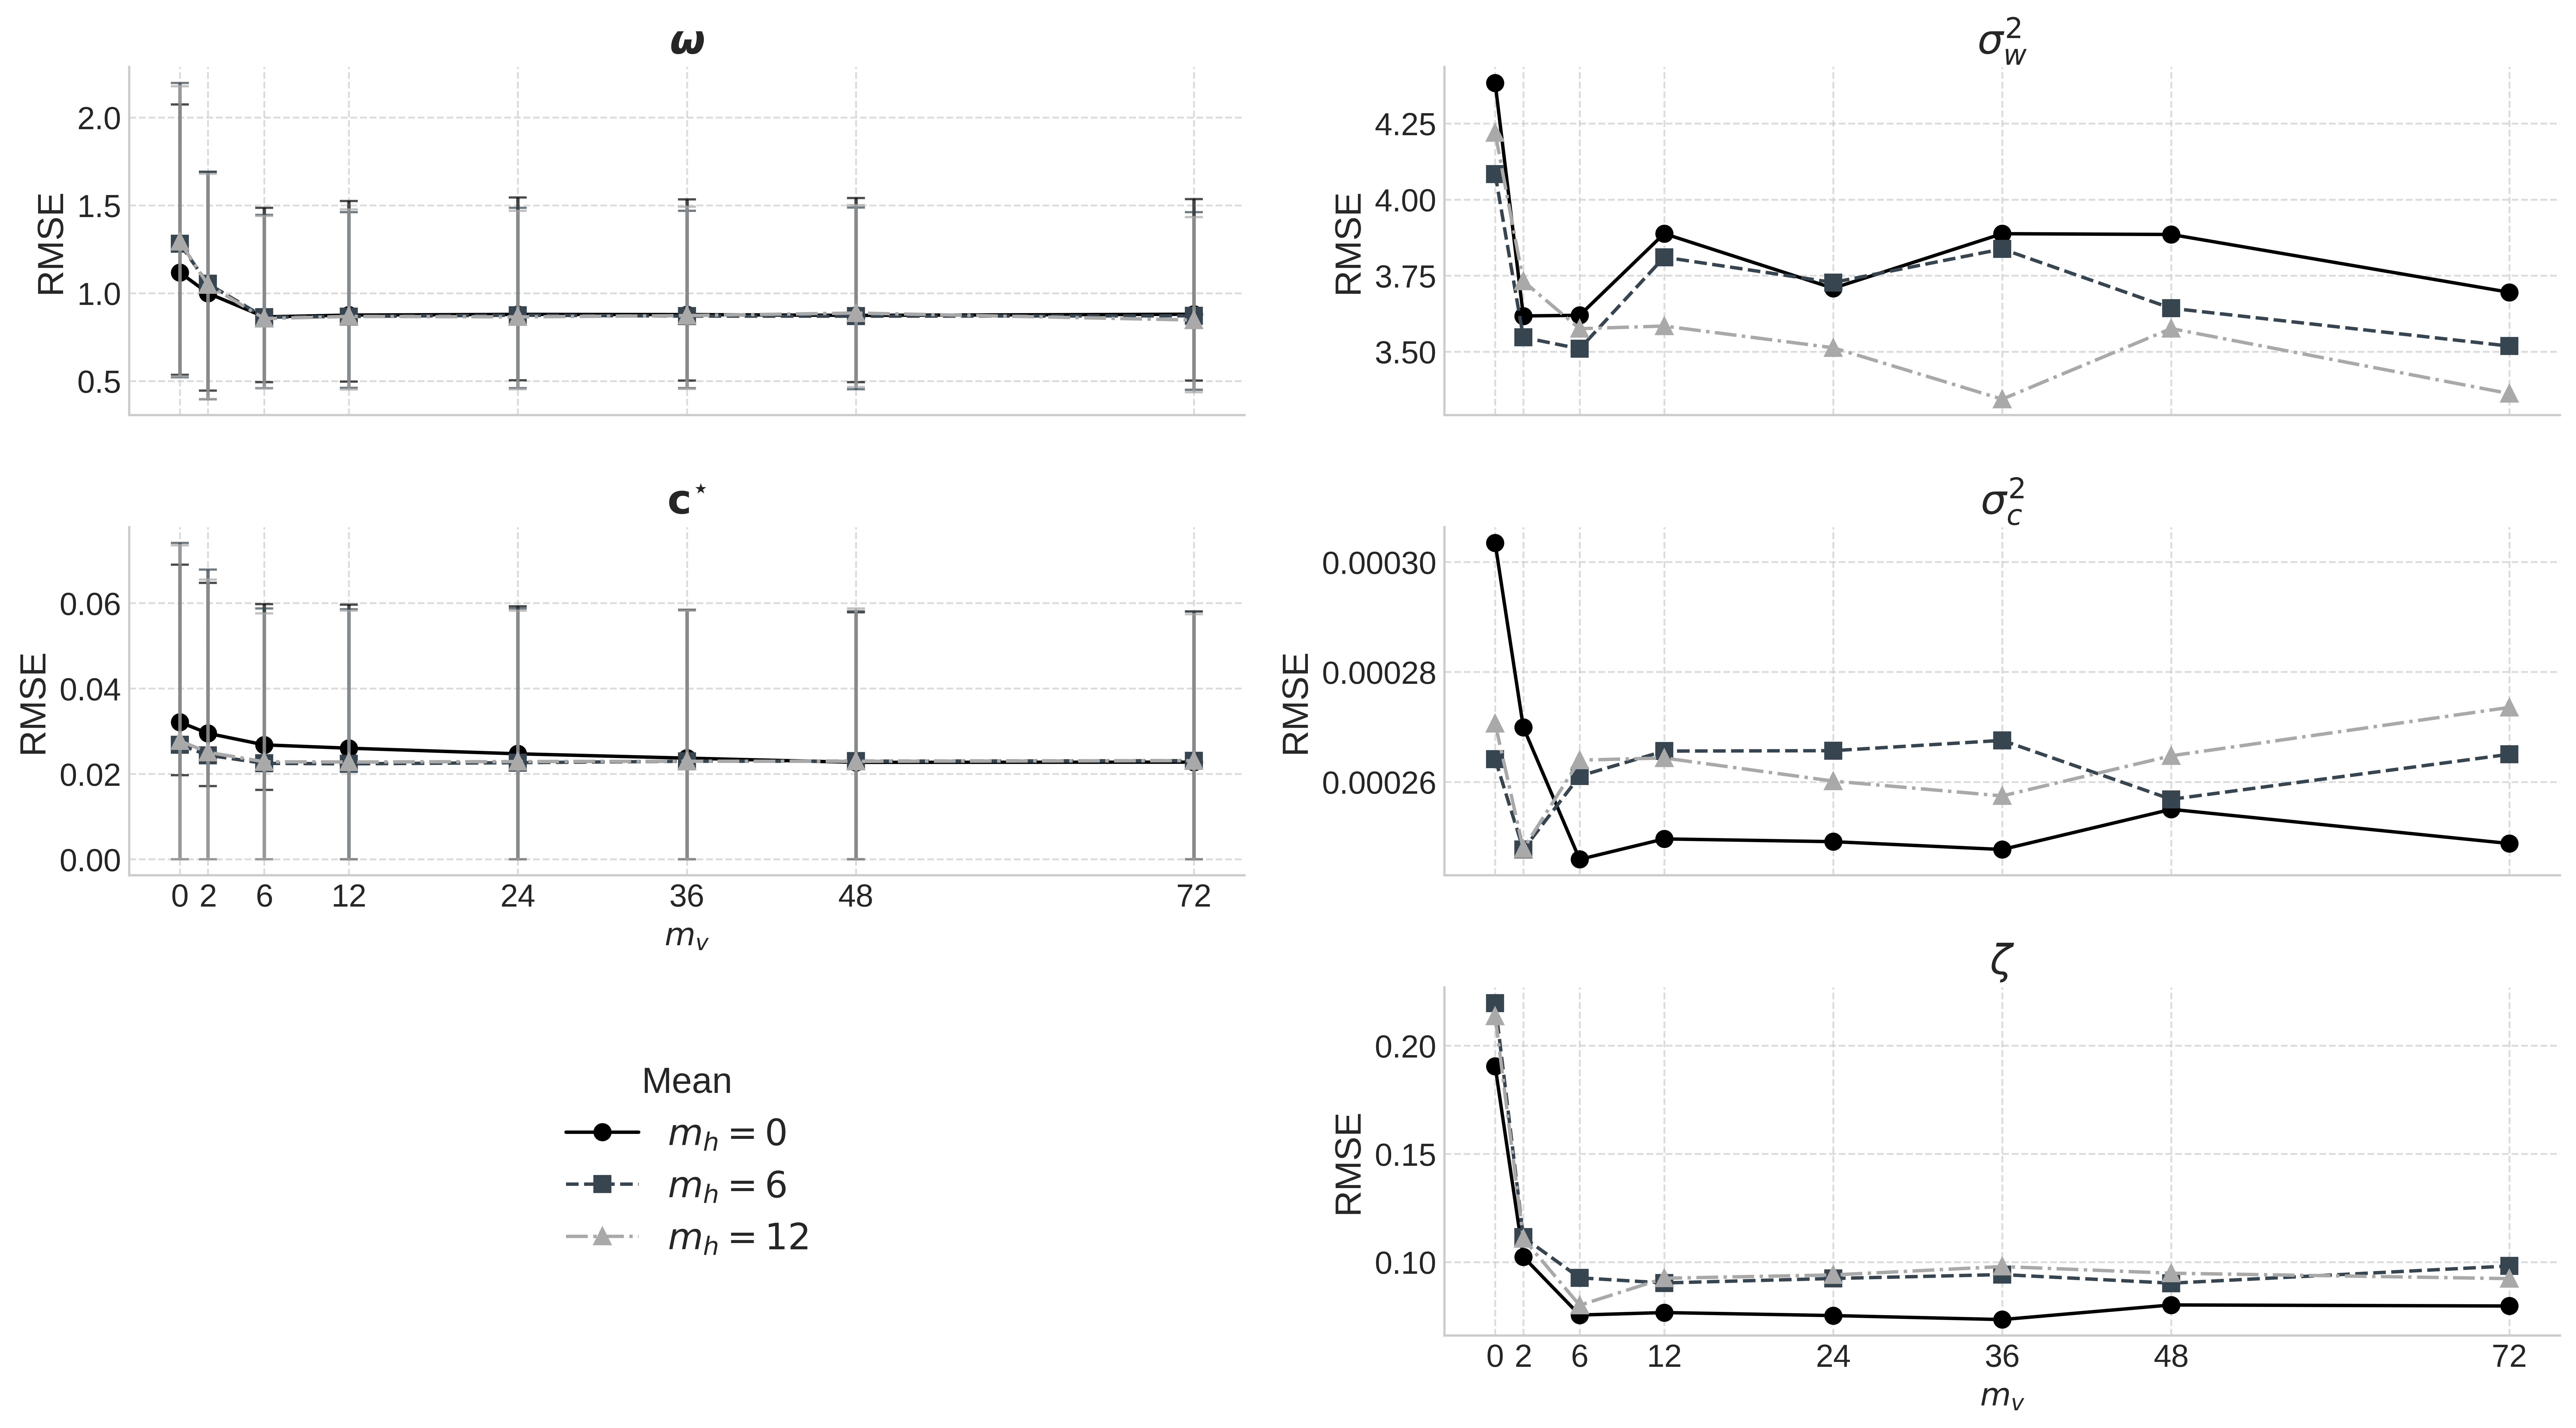
\includegraphics[width=\linewidth]{images/results/padding/rmse_margins_k12_example1_startTrue.jpeg}
    \caption{RMSE distribution of the multivariate parameters $\bm{\omega}$ and $\bm{c}_u^{\star}$ and scalar RMSE for the univariate parameters $\sigma_c^2$, $\sigma_w^2$, and $\zeta$ estimated from a simulated dataset. 
    Based on the plots for $\bm{\omega}$ and $\bm{c}_u^{\star}$, the RMSE stabilizes at $m_v= 12 = n_v^{\circ} / 2$ in the presence of horizontal padding, i.e. when $m_h \in \{ 6, 12\}$.}
    \label{fig:rmse_margin}
\end{figure}

{\spacingset{1}
\bibliography{bibliography.bib}
}
\end{document}